\documentclass[letterpaper,12pt,titlepage,oneside,final]{book}
%======================================================================
%   M A S C  T H E S I S
%======================================================================
%\documentclass[letterpaper,12pt,titlepage,openright,twoside,final]{book}

\newcommand{\package}[1]{\textbf{#1}} % package names in bold text
\newcommand{\cmmd}[1]{\textbackslash\texttt{#1}} % command name in tt font 
\newcommand{\href}[1]{#1} % does nothing, but defines the command so the

\usepackage[cmex10]{amsmath}
\usepackage{amssymb,amsfonts,amsopn}
\usepackage{algorithmic}
\usepackage{array}
\usepackage[tight,footnotesize]{subfigure}
\usepackage{ifthen}
\usepackage{listings}
\usepackage{color}
\usepackage{booktabs}
\newboolean{PrintVersion}
\setboolean{PrintVersion}{false} 

%\usepackage{nomencl} % For a nomenclature (optional; available from ctan.org)
\usepackage{amsmath,amssymb,amstext} % Lots of math symbols and environments
\usepackage[pdftex]{graphicx} % For including graphics N.B. pdftex graphics driver 

% Custom *.STY files:
\usepackage{sty/macros}
\usepackage{sty/cases}
\usepackage{sty/IEEEtrantools}
\usepackage[pdftex,letterpaper=true,pagebackref=false,colorlinks=false,linkcolor=black,anchorcolor=black,citecolor=black,filecolor=black,menucolor=black,runcolor=black,urlcolor=black]{hyperref}

\hypersetup{
    plainpages=false,       % needed if Roman numbers in frontpages
    pdfpagelabels=true,     % adds page number as label in Acrobat's page count
    bookmarks=true,         % show bookmarks bar?
    unicode=false,          % non-Latin characters in Acrobat’s bookmarks
    pdftoolbar=true,        % show Acrobat’s toolbar?
    pdfmenubar=true,        % show Acrobat’s menu?
    pdffitwindow=false,     % window fit to page when opened
    pdfstartview={FitH},    % fits the width of the page to the window
    pdftitle={Robust and Energetically Efficient Walking Control Strategy for Bipedal Robots},
    pdfauthor={Safwan Choudhury},
    pdfsubject={Systems and Controls}, 
    pdfkeywords={Bipedal Locomotion} {Robust Gait} {Bipedal Stability} {Humanoid Robotics}, 
    pdfnewwindow=true,      % links in new window
    colorlinks=true,        % false: boxed links; true: colored links
    linkcolor=black,        % color of internal links
    citecolor=black,        % color of links to bibliography
    filecolor=magenta,      % color of file links
    urlcolor=cyan           % color of external links
}

\definecolor{dkgreen}{rgb}{0,0.6,0}
\definecolor{gray}{rgb}{0.5,0.5,0.5}
\definecolor{mauve}{rgb}{0.58,0,0.82}

\lstset{    language=Matlab, 
            numbers=left,
            aboveskip=3mm,
            belowskip=3mm,
            showstringspaces=false,
            columns=flexible,
            basicstyle={\small\ttfamily},
            numberstyle=\tiny\color{gray},
            keywordstyle=\color{blue},
            commentstyle=\color{dkgreen},
            stringstyle=\color{mauve},
            breakatwhitespace=true
            tabsize=3
        }


\ifthenelse{\boolean{PrintVersion}}{   % for improved print quality, change some hyperref options
\hypersetup{	% override some previously defined hyperref options
%    colorlinks,%
    citecolor=black,%
    filecolor=black,%
    linkcolor=black,%
    urlcolor=black}
}{} % end of ifthenelse (no else)


% Set margins to minimum permitted by uWaterloo thesis regulations:
\setlength{\marginparwidth}{0pt}
\setlength{\marginparsep}{0pt}
\setlength{\evensidemargin}{0.125in}
\setlength{\oddsidemargin}{0.125in}
\setlength{\textwidth}{6.375in}

\raggedbottom
\setlength{\parindent}{0cm}
\setlength{\parskip}{\medskipamount}
\renewcommand{\baselinestretch}{1}
\let\origdoublepage\cleardoublepage
\newcommand{\clearemptydoublepage}{%
  \clearpage{\pagestyle{empty}\origdoublepage}}
\let\cleardoublepage\clearemptydoublepage

%======================================================================
%   T H E S I S  D O C U M E N T
%======================================================================
\begin{document}

    % F R O N T   M A T T E R
    %======================================================================
%   F R O N T  M A T T E R
%======================================================================
\pagestyle{empty}
\pagenumbering{roman}


% T I T L E   P A G E
% -------------------
\begin{titlepage}
    \begin{center}
        \vspace*{1.0cm}

        \Huge
        {\bf Design and Gait Synthesis for a \\ 3D Lower Body Humanoid}

        \vspace*{1.0cm}

        \normalsize
        by \\

        \vspace*{1.0cm}

        \Large
        Safwan Choudhury \\

        \vspace*{3.0cm}

        \normalsize
        A thesis \\
        presented to the University of Waterloo \\ 
        in fulfillment of the \\
        thesis requirement for the degree of \\
        Master of Applied Science \\
        in \\
        Electrical Engineering\\
 		Systems and Controls \\

        \vspace*{2.0cm}

        Waterloo, Ontario, Canada, 2012 \\

        \vspace*{1.0cm}

        \copyright\ Safwan Choudhury 2012 \\
    \end{center}
\end{titlepage}

\pagestyle{plain}
\setcounter{page}{2}

\cleardoublepage


% D E C L A R A T I O N
% ---------------------
\noindent
I hereby declare that I am the sole author of this thesis. This is a true copy of the thesis, including any required final revisions, as accepted by my examiners.

\bigskip
  
\noindent
I understand that my thesis may be made electronically available to the public.

\cleardoublepage
%\newpage


% A B S T R A C T
% ---------------
\begin{center}
    \textbf{Abstract}
\end{center}

\ifthenelse{\boolean{VoidIncomplete}}{\Incomplete}{
This is the abstract.
}

\cleardoublepage
%\newpage


% A C K N O W L E D G E M E N T S
% -------------------------------
\begin{center}
    \textbf{Acknowledgements}
\end{center}

I would like to thank my supervisor Dana Kuli\'{c} for her invaluable guidance and support throughout my research. I'm extremely grateful for her advice, paper editing, debugging sessions and countless meetings over the last two years.  

I would also like to thank the following people for their assistance during the course of my masters research: 

\begin{itemize}
    \item Dr. Derek Wight for his advice on electromechanical design, developing models with QUARC and help with the HIL experiments. I am also grateful for the opportunity to work at Quanser Inc under the NSERC Industrial Postgraduate Scholarship. The experience was extremely valuable to the development of our streamlined toolchain during the design process. \\

    \item Christopher Kirby from Christie Digital Systems for taking the time to to provide guidance on the mechanical design. As an electrical engineering undergraduate with minimal experience and knowledge of mechanical engineering, his advice on best  practices, designing the mechanical power transmission system for the biped and generating CAD drawings was invaluable. \\

    \item Matt Millard of the Real Motion Group in Systems Design Engineering for his expertise in the field of gait analysis and for help with a wide range of topics pertaining to walking robots and contact modeling.  \\

    \item Charles Boyle at the Engineering Machine Shop on campus for his advice and assistance with manufacturing the bipedal robot. Charlie often stayed after hours and helped with machining various parts of the project.  \\

\end{itemize}

Finally, I would like to thank my family and my wife for providing their endless encouragement and support throughout my academic career at the University of Waterloo. 

\cleardoublepage
%\newpage


% D E D I C A T I O N
% -------------------
% \begin{center}
%     \textbf{Dedication}
% \end{center}

% This is dedicated to the one I love.
% \cleardoublepage
%\newpage


% T A B L E   O F   C O N T E N T S
% ---------------------------------
\renewcommand\contentsname{Table of Contents}
\addcontentsline{toc}{chapter}{Table of Contents}
\tableofcontents
\cleardoublepage
\phantomsection
%\newpage


% L I S T   O F   T A B L E S
% ---------------------------
\addcontentsline{toc}{chapter}{List of Tables}
\listoftables
\cleardoublepage
\phantomsection		% allows hyperref to link to the correct page
%\newpage


% L I S T   O F   F I G U R E S
% -----------------------------
\addcontentsline{toc}{chapter}{List of Figures}
\listoffigures
\cleardoublepage
\phantomsection		% allows hyperref to link to the correct page
%\newpage


% L I S T   O F   S Y M B O L S
% -----------------------------
% To include a Nomenclature section
% \addcontentsline{toc}{chapter}{\textbf{Nomenclature}}
% \renewcommand{\nomname}{Nomenclature}
% \printglossary
% \cleardoublepage
% \phantomsection % allows hyperref to link to the correct page
% \newpage

\pagenumbering{arabic} % Change page numbering back to Arabic numerals

 

    % T H E S I S   C H A P T E R S
    \chapter{Introduction} % (fold)
\label{cha:introduction}
Bipedal locomotion is a highly active research area within the field of humanoid robotics. As robotics continue to push towards becoming more mainstream, the ability for a robotic system to navigate an environment designed for humans is essential for them to be useful. However, bipedal locomotion is a very challenging control problem due to the natural instability of a dynamic and nonlinear system. Over the past 40 years, most control strategies have focused around using a measure of balance to come up with walking control algorithms. However, the downside thus far has been energetically inefficient gait which is very ``robot-like''. 

In this thesis, we present a novel walking control strategy which is energetically efficient and robust to external disturbances. However, a key challenge in validating most control approaches in the field of humanoid robotics is validating simulations with physical hardware. To this end, this thesis outlines the construction of a 14 degree-of-freedom (DOF) lower body humanoid robot for the purposes of research in bipedal locomotion. The ultimate goal is to apply the walking control strategy on the bipedal robot and validate the effectiveness and usefulness of the presented walking control strategy. 

\section{Contributions} % (fold)
\label{sec:contributions}
At the very core of the proposed walking control strategy is the Foot Placement Estimator (FPE) algorithm which has been presented for 2D bipedal robots. Simply put, the FPE algorithm determines where an unstable bipedal robot must step to regain balance. The elegance of this approach lies in the fact that it can be extended to form complete gait cycles in the 2D case using simple PD controllers and a state machine. 

In this thesis, the 2D FPE theory is extended to form complete gait cycles for a 3D bipedal robot in simulation and ultimately, on physical hardware. Extending the 2D theory presents its own unique set of challenges which are addressed in part using prioritized whole body motion control. Ultimately, the efficacy of the proposed walking control strategy is demonstrated in simulation. The physical 14 DOF bipedal robot is constructed but due to time limitations, only the validity of the motion control framework is demonstrated on physical hardware. 
% section contributions (end)

\section{Outline} % (fold)
\label{sec:outline}
The remainder of this thesis is organized as follows. Chapter \ref{cha:background} outlines existing walking control strategies prevalent in literature today. While most control strategies use a dynamic measure of balance to form complete gait cycles, some newer approaches are similar to the strategy presented in this thesis. That is, these control strategies aim to use foot placement as a means to form robust and energetically efficient gait for bipedal locomotion. 

One of the key challenges in developing physical hardware for bipedal locomotion research is the impact of small changes in the electromechanical design on the overall stability of the system. In order to effectively develop a system with adequate drivetrain performance to achieve walking, a toolchain is developed to streamline the process of designing a mechanical prototype in CAD and immediately analyzing its behaviour in dynamic simulations. The electromechanical design workflow using the toolchain is presented in Chapter \ref{cha:toolchain}. 

Extending the current 2D FPE theory to the 3D case is presented in Chapter \ref{cha:simulations}. A prioritized whole body motion control scheme is presented in order to simultaneously use the FPE algorithm to achieve walking and maintain stability throughout the entire gait cycle. The 2D FPE theory and the proposed extension to 3D are both verified in dynamic simulations. 

Next, the electromechanical design of a 14 DOF lower body humanoid robot is presented in Chapter \ref{cha:design}. Human gait is used as an approximate starting point for actuators and drivetrain component selection from local vendors. The forward dynamics and 3D visualization for the final prototype design is generated using the toolchain outlined in in Chapter \ref{cha:toolchain}. This is used to test control strategies on the 14 DOF lower body humanoid platform in simulation prior to implementing it on the physical hardware. 

Experimental validation of the drivetrain dynamics and whole body motion control frameworks are validated on the physical hardware in Chapter \ref{cha:experiments}. The actuator dynamics models in simulation are verified to match the physical DC motors through hardware-in-the-loop (HIL) simulations. The whole body motion control framework used for extending the FPE theory to 3D is also verified on physical hardware using HIL.  

Lastly, conclusions and future work regarding the proposed walking control strategy and developed physical hardware are presented in Chapter \ref{cha:conclusion}. 
% section outline (end)

% chapter introduction (end) 
    \chapter{Related Work} % (fold) ===============================================
\label{cha:background}
Bipedal locomotion is one of the most active areas of research within humanoid robotics. This section presents a brief literature review on the design and gait synthesis for humanoid robotic applications. 



%==============================================================================
%   E L E C T R O M E C H A N I C A L   D E S I G N 
%==============================================================================



\section{Humanoid Electromechanical Design} % (fold) ==========================
\label{sec:related_electromechanical_design}
The electromechanical design of humanoid robots have undergone several generations of revisions. 


\subsection{Degrees of Freedom} % (fold) ======================================
\label{sub:related_degrees_of_freedom}
The selection of degrees-of-freedom (DOF) of a humanoid robot plays an essential role in the design and development phase. 
% subsection degrees_of_freedom (end) =========================================


\subsection{Mechanism Design} % (fold) ========================================
\label{sub:related_mechanism_design}
Linkage subsystems used to carry out motion is also an area where several approaches exist. 
% subsection mechanism_design (end) ===========================================


\subsection{Passivity-Based Designs} % (fold) =================================
\label{sub:related_passive_designs}
Perhaps the simplist approach to designing bipedal robots are those without any active power. 
% subsection passivity_based_designs (end) ====================================


\subsection{Actively-Powered Designs} % (fold) ================================
\label{sub:related_active_designs}
The most common approach to electromechanical design for bipedal robots is through the generation of active power for locomotion. 
% subsection actively_powered_designs (end) ===================================


% section humanoid_electromechanical_design (end) =============================



%======================================================================
%   W A L K I N G  C O N T R O L  &  G A I T  G E N E R A T I O N
%======================================================================



\section{Walking Control Strategies and Gait Generation} % (fold) =============
\label{sec:related_control_strategies}
There exists a wide range of control strategies to achieve bipedal locomotion in robotics literature to date. Some of the most popular strategies are briefly reviewed in this section.


\subsection{Zero-Moment Point} % (fold) =======================================
\label{sub:related_zero_moment_point}
The most popular techniques to achieve walking have been trajectory generation and control strategies based on the Zero-Moment Point (ZMP) criterion \cite{Vukobratovic:2004wy}. The ZMP defines a point on the ground where the forces acting on a biped do not produce a moment about the axes parallel to the ground plane. If the ZMP is kept within the region of foot support, the biped is stable. This stability criterion can be used to compute ZMP-stable trajectories offline that maximize the stability margin by maximizing the distance from the ZMP to the boundary of the support region. In the on-line phase, the stable trajectories are tracked online to execute walking \cite{HuangEtAlTRA2001}.  ZMP-based trajectories can also be generated on-line \cite{KajitaEtAlICRA2003,TakenakaEtAlIROS2009}. 

One of the biggest drawbacks of this approach is the resulting trajectory does not provide any strategy to respond to disturbances due to uneven terrain or unexpected forces. Typically, these strategies \cite{Kajita:1997vr,Kajita:2001fk,Sugihara:2002kq} are also energetically inefficient since they are constantly trying to maintain balance by keeping the ZMP point within the region of foot support. Furthermore, the resulting gait does not utilize the natural dynamics of the system and consequently does not look human-like. Despite the drawbacks, some of the most popular humanoid robots today utilize some variation of ZMP based feedback for bipedal locomotion. The most popular application is the famous Honda Asimo \cite{Hirai1998}. Newer bipeds available for research like Aldebaraan's Nao \cite{Gouaillier2006} robot also use ZMP-based walking control strategies. 
% subsection zero_moment_point (end) ==========================================


\subsection{Passive Dynamics} % (fold) ========================================
\label{sub:related_passive_dynamics}
An alternative approach, first proposed by McGeer \cite{McGeer:1990uk}, introduced a unique class of legged robots known as passive dynamic walkers \cite{Collins:2005vp}. This approach takes advantage of the natural dynamics of the biped structure, and is capable of maintaining a stable gait cycle without active control effort. Fully passive mechanisms walk on an inclined surface so that the mechanism is powered by gravity alone \cite{Spong:1999vk}. In addition to producing highly efficient walk, the gait patterns generated using this approach appear more human-like in comparison to ZMP-based control. However, passive dynamic walkers lack robustness to perturbations due to very narrow regions of attraction.

Thus far, majority of the research in passive dynamics has been restricted the very specific scenario of walking on an incline. This lacks the versatility that is required for humanoid robots if they are to ultimately navigate in most human environments (level ground). Further investigative research was helpful in characterizing the nature of a passive gait cycle \cite{Goswami:1996gn} in terms of stability and energies. This ultimately gave rise to new strategies which were aimed towards emulating the work done by gravity on an inclined slope \cite{Asano:2000wi}. These hybrid approaches known as virtual passive dynamics improved the versatility of the simple legged robots to walk on level ground with minimal actuation as a replacement for gravity \cite{Asano:2004tv}. 

While these minimally actuated bipeds have been shown to exhibit similar energetics as purely passive machines \cite{Asano:2004jp}, most research is typically restricted to 2D dynamics in the sagittal plane. The challenges of extending these simple models to 3D (i.e. incorporating lateral dynamics) lies in the unstable motion introduced by mismatch of roll velocity and contact conditions \cite{Kuo:1999tn}. This is particularly challenging since even small disturbances can be completely destabalizing for passive dynamic walkers. Although the minimal actuation strategy based on passive dynamics is more versatile, the main difference between the two approaches simply boils down the source of energy used for walking. Regardless of the source, the quantity of energy provided stay within a stable limit cycle depends only on the slope of the incline \cite{Goswami:1996gn}. Thus, stabilizing the dynamics in both sagittal and frontal planes is particularly challenging since both strategies share the same underlying weakness to perturbations. 
% subsection passive_dynamics (end) ===========================================


\subsection{Force/Impedance} % (fold) =========================================
\label{sub:related_force_impedance}
\Incomplete
% subsection force_impedance_control (end) ====================================


\subsection{Machine Learning} % (fold) ========================================
\label{sub:related_machine_learning}
\Incomplete
% subsection machine_learning_strategies (end) ================================


\subsection{Foot Placement} % (fold) ==========================================
\label{sub:related_foot_placement}
Recently, an alternative problem formulation focusing on restoring balance has been proposed. The Foot Placement Estimator (FPE), introduced by Dwight et al \cite{Wight:2008ii} formulates an approach to restore balance by controlling swing foot position during the gait cycle. By using the conservation of angular momentum, the FPE equation determines the location on the ground where the total energy of an unstable biped after swing foot impact is equal to the peak potential energy. If a step is taken before the FPE location, the post impact energy of the system causes the biped to fall over. Conversely, stepping beyond the FPE location on the ground causes the biped to fall back onto the hind leg.

The solution to the FPE equation itself can be used as a recovery mechanism (i.e. in the face of a destabilizing disturbance) with existing ZMP-based strategies. Alternatively, it can be used to increase the narrow regions of attraction which plague minimally actuated passive dynamic walkers \cite{Goswami:1996gn,Asano:2000wi,Kuo:1999tn}. The key concept here is that the FPE-based integration would require minimal joint actuation only to align a swing food appropriately to recover from a potential fall. As shown in \cite{Wight:2008ii,Wight:2008vt}, FPE can also be extended to form complete gait cycles to achieve dynamically stable walking. However, there are several key assumptions which are violated when attempting to implement this approach on a physical 3D robot. Namely, the theory presented in the derivations assume that the legs are massless and it only deals with the 2D dynamics in the sagittal plane.

The capture point concept, developed by Pratt et al. \cite{Pratt:2006vy}, is conceptually similar to the FPE. While the derivation of FPE is based on a simple compass biped model with fixed parameters, the capture point theory was derived using complex motion models which included using a flywheel body to control/offset any disturbances through the use of rotational inertia. Ultimately, the simplicity of the model allowed the FPE theory to be extended to complete gait cycles, while the work presented by Pratt et al simply solved the problem of lateral stabilization \cite{Wight:2008ii}.

Recently, a more comprehensive approach using the capture point for foot placement as a means to develop full walking control strategies has been proposed. De Boer \cite{DeBoer:2012wp} focused on the ground/foot interaction to develop a robust and energetically efficient walking control strategy for a force-controlled compliant lower-body biped. While this approach is philosophically similar to the idea behind FPE, there are several key differences. The approach presented in this thesis uses simple local controllers to form complete gait cycles and can be used on position-controlled joints without any complex actuation systems. The capturability framework demonstrated in \cite{Pratt01092012} used separate controllers for the swing and stance legs whereas this approach uses a single global differential kinematic resolution for whole body motion control.
% subsection foot_placement_strategies (end) ==================================


% section walking_control_strategies_&_gait_generation (end) ==================



%======================================================================
%   2 D  F O O T  P L A C E M E N T  E S T I M A T O R
%======================================================================




% chapter background (end) ====================================================
    \chapter{Electromechanical Design} % (fold)
\label{cha:design}

This chapter presents the electromechanical design of the 14 DOF bipedal robot. There are several key design considerations which impact the performance of the finished product. The complete process consisted of selecting the appropriate drivetrain components (electric machines) and designing the mechanical chassis. The primary design objective was to produce enough mechanical power for the robot to achieve walking. The secondary design objective was to keep the overall weight low and raise center of mass (COM) position as high as possible. 

The initial design specification was obtained by modeling the system dynamics and gait estimation (Section~\ref{sec:designspec}). The selection of electromechanical components which compose the drivetrain system was used to address the primary design objective (Section~\ref{sec:drivetrain}). These drivetrain components include electric machines (DC motors) and adequate gearing which provide the reduction ratio required to meet the initial design specifications. After the primary objective was addressed and the drivetrain components were selected, the secondary design objectives were satisfied by adjusting the mechanical structure and manipulating placement of components (Section~\ref{sec:chassis}).

%======================================================================
%   D Y N A M I C  M O D E L I N G
%======================================================================

\section{Dynamic Modeling} % (fold)
\label{sec:designspec}

A dynamic model of the proposed system must be developed and analyzed under normal operating conditions to determine the effect of forces acting on the system and torques experienced at each of the joints. The forward or direct dynamic model is a mathematical system which provides a transformation from the joint torques to the resulting joint positions, velocities and accelerations. That is, it provides the mapping:

\begin{equation}
	\ddot{\vec{q}} = f(\vec{\tau})
\end{equation}

Given this model, a dynamic simulation environment can be designed to estimate the torque loading at different joints on the bipedal robot during the gait cycle. This estimate can form the basis of the initial design specifications from which motors and gearing can be selected. An important consideration in this model is the inclusion of contact forces during the stance phase of the gait cycle. The ground reaction forces exerted on the robots feet have a significant impact on the dynamic requirements of each joint. Since the stance phase makes up approximately 60\% of the gait cycle, the effects these forces have to be incorporated for an accurate simulation. 
% section overview (end)

\subsection{Equations of Motion} % (fold)
\label{sec:forward_dynamics}

The general form of the equation of motion describing a $n$-DOF humanoid robot (with a floating base) is given by: 

\begin{equation}
	\label{eq:eom1}
	A(\vec{q})\ddot{\vec{q}} + C(\vec{q},\dot{\vec{q}})\dot{\vec{q}} + g(\vec{q}) = \vec{\tau}
\end{equation}

Where $A(\vec{q})$ is the $(n+6) \times (n+6)$ inertia matrix, $C(\vec{q},\dot{\vec{q}})$ are the centripetal/Coriolis terms and $g(\vec{q})$ is the gravity vector. The $(n+6) \times 1$ generalized force vector $\vec{\tau}$ is segmented as follows:

\begin{equation}
	\label{eq:gentau}
	\vec{\tau} = {\begin{bmatrix} \vec{\tau_{act}} & \vec{\tau_{base}} \\ \end{bmatrix}}^T
\end{equation}

Where $\tau_{act}$ represents the $n$ actuated DOF and $\tau_{base} = \bf{0}_{6 \times 1} $ are the remaining non-actuated DOF at the floating base. In order to incorporate the effects of contact forces at both feet of the biped robot, (\ref{eq:eom1}) is modified as follows: 

\begin{equation}
	\label{eq:eom2}
	\begin{bmatrix} A_{11} & A_{12} \\ A_{21} & A_{22} \end{bmatrix} 
	\begin{bmatrix} \ddot{\vec{q}}_{act} \\ \ddot{\vec{q}}_{base} \end{bmatrix} + 
	\begin{bmatrix} b_{1} \\ b_{2} \end{bmatrix} = 
	\begin{bmatrix} \vec{\tau_{act}} \\ 0 \end{bmatrix} + 
    J^{T}\vec{F}_{left} + J^{T}\vec{F}_{right}
\end{equation}

Where the generalized acceleration vector $\ddot{q}_{act}$ represents the $n$-DOF joint motion and $\ddot{q}_{base}$ is for the 6 DOF base motion. The gravitational and Coriolis terms are combined into the $\vec{b}$ vector. Finally, $J$ is a 6 x $n$ Jacobian matrix provides the mapping between the joint space and work space. The force vectors $\vec{F}_{left}$ and $\vec{F}_{right}$ represent the contact force felt at the left and right foot, respectively. With this modification of the equation of motion, the external forces felt during the stance phase can be incorporated into the dynamic model of the overall system. The method of calculating the magnitude of the force itself depends on the contact model used for the system. Equation (\ref{eq:eom2}) represents the complete dynamics of the 14 DOF bipedal robot with $n = 14 + 6 = 20$ generalized coordinates.
% section forward_dynamics (end)

\subsection{Recursive Newton-Euler} % (fold)
\label{sec:kajita_s_matlab_toolbox}

One method of computing a direct dynamic model for the biped robot is through the use of the Recursive Newton-Euler (RNE) algorithm. This algorithm computes the inverse dynamics model iteratively in order to arrive at a final solution for the direct dynamics \cite{Perrin:1997wn}. The algorithm serially traverses through the kinematic chain to perform calculations using Newtonian mechanics. The first pass of the algorithm starts at the base link and traverses down the serial chains of the left and right legs calculating the kinematics. The second pass starts at the end of the serial chain(s) and works back up to the base link calculating the effect of dynamics. After the final pass, the RNE algorithm produces the torques at each joint and the 6 dimensional forces and moments felt by the (floating) base joint. The RNE algorithm reformulates the equation representing the complete dynamics of the system (\ref{eq:eom2}) to obtain the direct dynamics model. 
% The pseudocode listed in Appendix \ref{sec:rne_direct_dynamics} describes the procedure for computing the direct dynamics model by utilizing the RNE formulation.

Professor Shuuji Kajita packages a simple MATLAB \cite{sw:matlab} toolbox with his textbook on humanoid robotics \cite{kajitatxt} which was used as a starting point for the direct dynamics model to obtain initial design specifications. The toolbox provides preprogrammed routines for common robotics algorithms (i.e. forward/inverse kinematics, etc). The kinematic and dynamic parameters of the robot is defined in a global structure variable called \texttt{uLINK}. The packaged scripts and functions access key information (i.e. kinematic hierarchy of links) from the global struct to perform the calculations. An external application was developed to interface with the CAD software package's application programming interface (API) to extract the kinematic and dynamic parameters directly. The application used the extracted data to automatically generate the CAD-equivalent \texttt{uLINK} representation in MATLAB code (shown in Figure~\ref{fig:ulinkdrawn}).

\begin{figure}[!ht]
	\begin{center}
    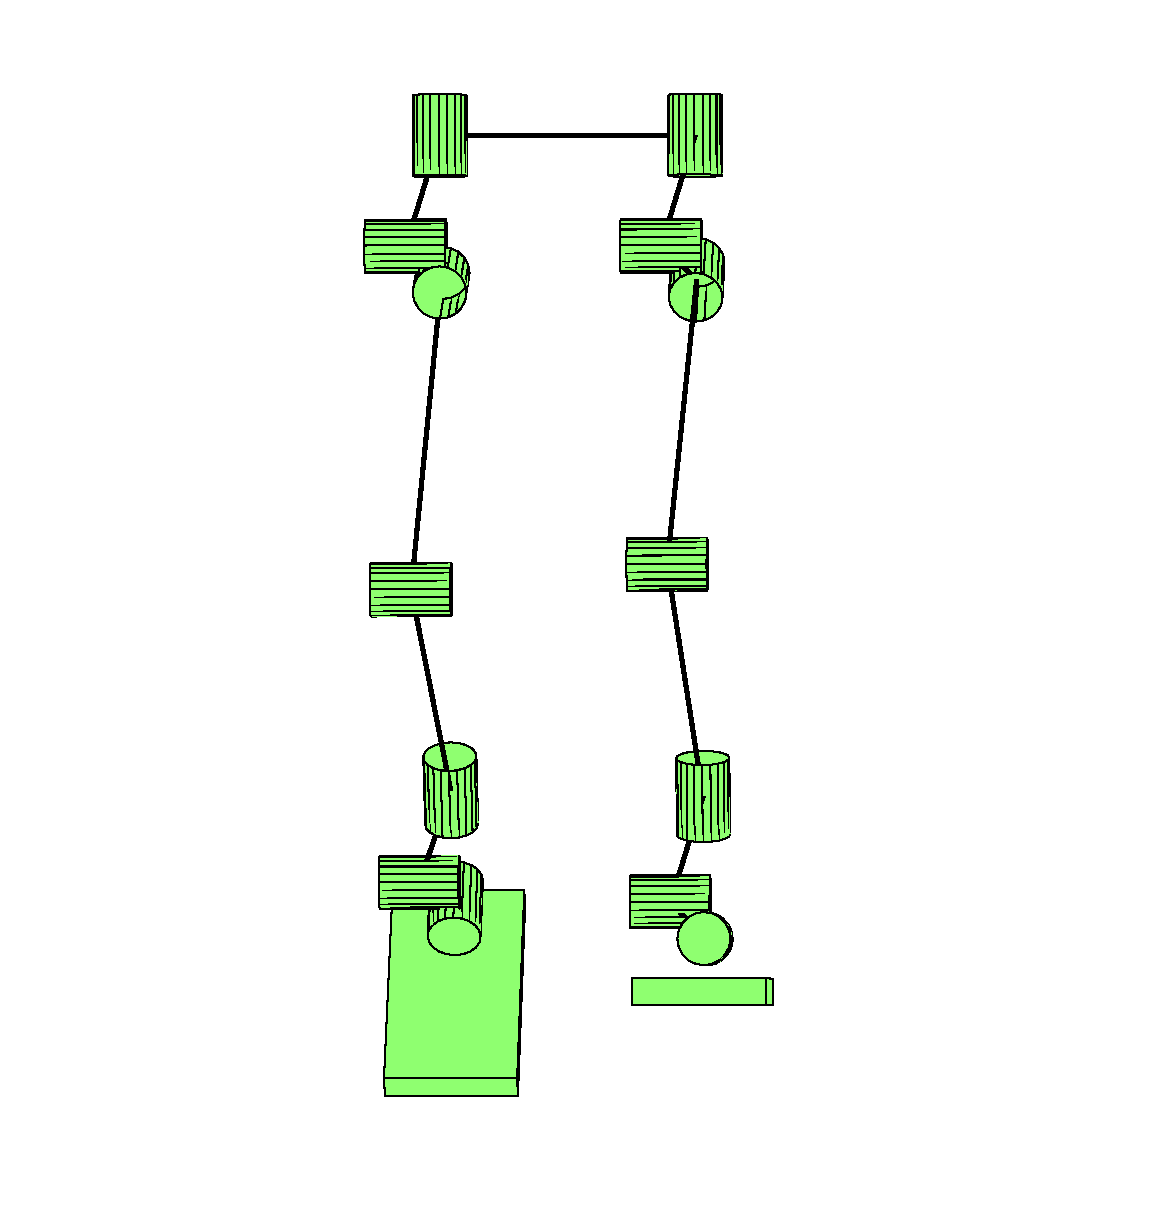
\includegraphics[scale=0.6]{fig/design/ulinkdrawn.eps}
	\end{center}
  \caption{Screenshot of robot structure drawn from uLINK definition generated directly from CAD.}
  \label{fig:ulinkdrawn}
\end{figure}

With the \texttt{uLINK} structure is generated, any of the preprogrammed routines in the toolbox can be used. The toolbox provides a function \texttt{ForwardDynamics} to compute the direct dynamics model using the RNE algorithm. However, the calculations omit the effects of any external forces acting on the system. Since it is important to incorporate the contribution of the ground reaction forces, the toolbox was modified to model the complete dynamics of the system. 

\subsection{Contact Modeling} % (fold)
\label{sub:initial_contact_modeling}

One challenging aspect of dynamic simulations is to accurately model the effects of external forces on the system during the stance phase. To emulate the ground reaction forces during this period of the gait cycle, a contact model is used to generate an approximate contact force. For the initial design specifications, a spring-damper contact model is used (shown in Figure~\ref{fig:springdamper}). Both feet are modelled as point contacts which experience a normal force proportional to the output of the spring-damper system when in contact with the ground. A more complex version of (\ref{eq:contactf}) is used for full dynamic simulations in later chapters (specifically in Section~\ref{sub:full_contact_modeling}).

\begin{figure}[!h]
	\begin{center}
    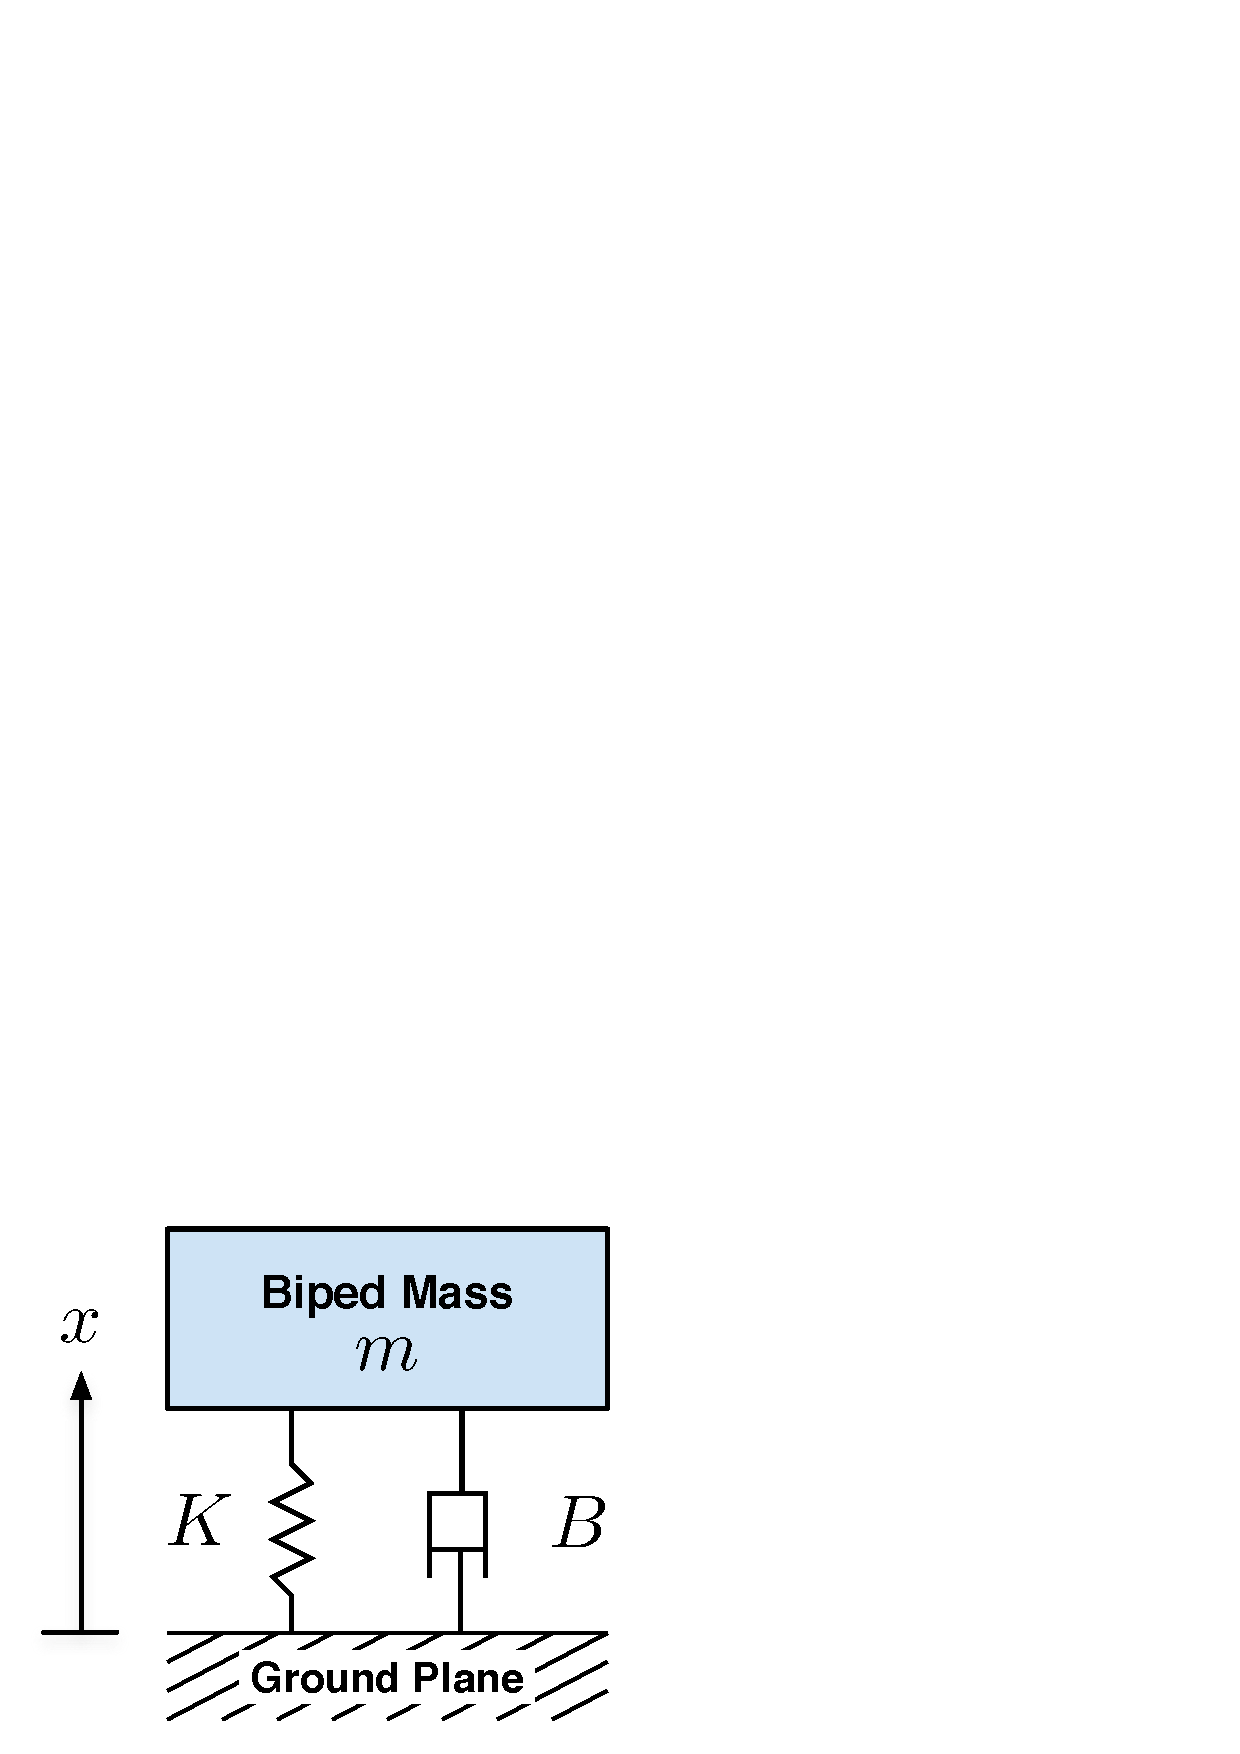
\includegraphics[width=100mm]{fig/design/springdamper.png}
	\end{center}
  \caption{System diagram of spring-damper contact model used in dynamic simulations.}
  \label{fig:springdamper}
\end{figure}

To incorporate the effects of ground contact into the existing dynamic model, the resulting force produced by (\ref{eq:contactf}) is injected into the RNE algorithm between the end of the first pass and the start of the second pass. At the start of the second pass, the external contact force is used to initialize the backwards recursion. Due to the serial nature of RNE, this force traverses up the kinematic chain(s) for each leg and is ultimately resolved at the base. Alternatively, the equivalent force can be substituted into the overall system dynamics represented in Equation \ref{eq:eom2} for $F_{left}$ and $F_{right}$. Both approaches will yield identical results as the contact force is resolved into each joint of the biped robot. 

\begin{equation}
	\label{eq:contactf}
	\vec{F}_{contact} = B\vec{\dot{x}} + K\vec{x}
\end{equation}

Since the direct dynamics routine packaged with Professor Shuuji Kajita's toolbox is based on the RNE algorithm, the modication required to incorporate the contact model was minimal. The contact force proportional to the output of the spring-damper system was used to initialize the backwards pass as shown below: 

\lstinputlisting{code/kajitamod.m}

Where the variables \texttt{Kr} and \texttt{Br} represent the spring and damper coefficients in the spring-damper contact model. \texttt{RCONTACT} is simply a constant link number representing the point contact foot. The velocity due to the point foot coming in contact with the ground (\texttt{vr}) is recomputed by considering the original velocity (\texttt{vo}) and the cross product between the position of the foot (\texttt{uLINK.p}) and angular velocity (\texttt{uLINK.w}). The resulting normal force is computed and injected into the backwards pass if the foot position is below the ground level (condition shown in line 1). With this modification included, the complete direct dynamics can be used to obtain the joint torques during an estimated gait cycle for the initial design specification.   
% subsection modifications (end)

% section contact_modelling (end)

% section kajita_s_matlab_toolbox (end)

\subsection{Gait Estimation} % (fold)
\label{sec:gait_estimation}
	
In order to emulate the operating conditions for the 14 DOF bipedal robot once it is built, the dynamic simulation must include all dynamic effects experienced during a complete gait cycle. One method of emulating the normal operating conditions to use human gait as an estimate. While it is ambitious to expect a bipedal robot to match the performance of human-like walking, it provides a basis from which the initial selection of electromechanical components can emerge. The goal is to extract the kinematic parameters experienced by the human limbs while walking and impose similar conditions on the robot in dynamic simulation. Given these constraints, the inverse dynamics problem can be solved to obtain the joint torque estimates during various stages of the gait cycle. Coupled with the modifications to emulate contact forces during the stance phase, this approach provides a fast method of estimating the torque loading at each joint to develop the initial design specification. 
	
In order to use kinematic parameters from human gait, data published from the 2008 Dynamic Walking conference was used \cite{dw2008}. The published dataset used sensors to measure the joint angles and velocities of lower body human limbs under several gait cycle speeds (fast, slow walk and normal walk). During the data collection, sensors were strategically placed such that key information such as the knee and hip pitch joint angles were captured. This raw sensory data was imported into the MATLAB environment using a 3D motion analysis toolbox BodyMech \cite{bodymech}. This information was incorporated into the dynamic simulation by enforcing the joint angles, velocities and accelerations from each captured frame of the reference dataset. The forced joint parameters were assigned to the global \texttt{uLINK} structure to be used in conjunction with the RNE-based inverse dynamics algorithm. 

\begin{figure}[!h]
	\begin{center}
	\begin{tabular}{cc}
	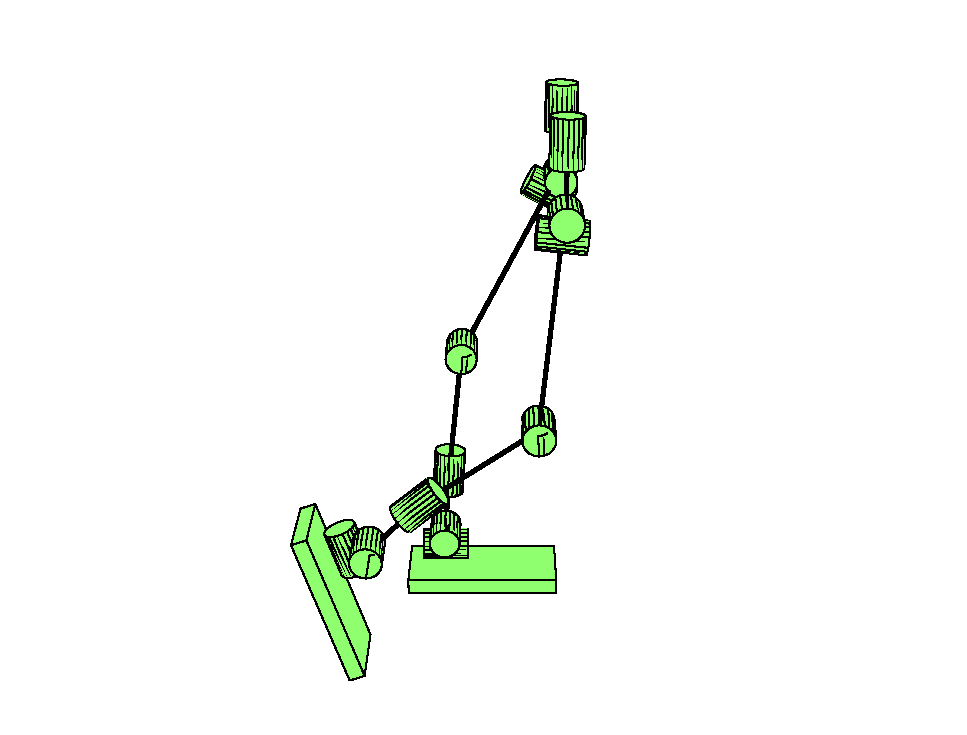
\includegraphics[scale=0.5]{fig/design/ulinkwalk1.eps} &
    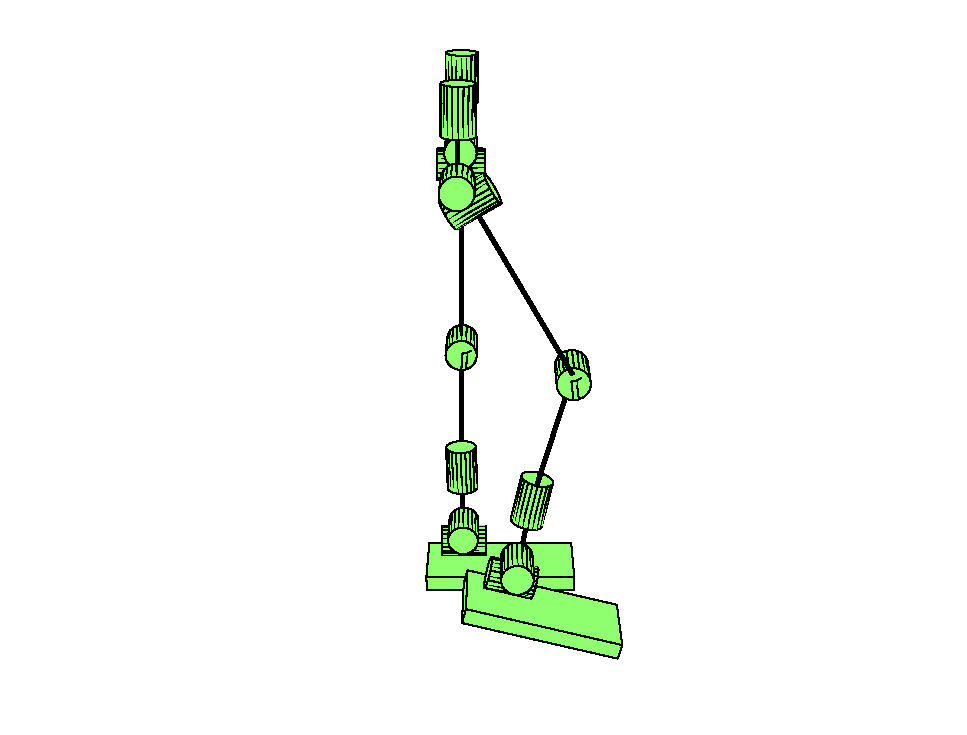
\includegraphics[scale=0.5]{fig/design/ulinkwalk.eps}
	\end{tabular}
	\end{center}
  \caption{Frame captures of the uLINK structure under the estimated gait cycle to obtain initial design specifications.}
  \label{fig:ulinkframes}
\end{figure}

An experiment was devised in the MATLAB environment which used a combination of the BodyMech toolbox and Professor Shuuji Kajita's toolbox. The BodyMech toolbox was used to extract the frame-by-frame 3D kinematic parameters as a human executed the gait cycle. These parameters were processed and stored in order to be played back on the robot model defined by the \texttt{uLINK} structure. To compensate for the differences in size between humans and the small biped, the joint velocities and accelerations were scaled by selecting a different reference gait speed from the published data set. Once the parameters were applied, the RNE-based inverse dynamics algorithm was used to determine the torques at each joint in the structure as result of the estimated gait. This process was repeated for each frame (illustrated in Figure~\ref{fig:ulinkframes}) in the captured dataset and the results of robots kinematics/dynamics ($\vec{q}$, $\vec{\dot{q}}$, $\vec{\ddot{q}}$ and $\vec{\tau}$) were tabulated for post processing. 
% section gait_estimation (end)


\subsection{Initial Design Specifications} % (fold)
\label{sec:initial_design_requirements}
The results of the dynamic simulations under human-gait analysis form the basis for the initial electromechanical components selection process. As expected, it was observed that the largest demands in torque loading on each of the joints occurred during the stance phase immediately after the heel strike (refer to Frame 36 in Figure \ref{fig:gaitplot}). The torque demands at that instant spike immediately to almost 3x the steady state torque loading on the joints. While it is expected that a walking robot will experience large spikes in the torque demands such as the ones observed in the dynamic simulation, it is unreasonable to use only the peak torque values as the required specifications for design. 

\begin{figure}[!h]
	\label{fig:gaitplot}
	\begin{center}
    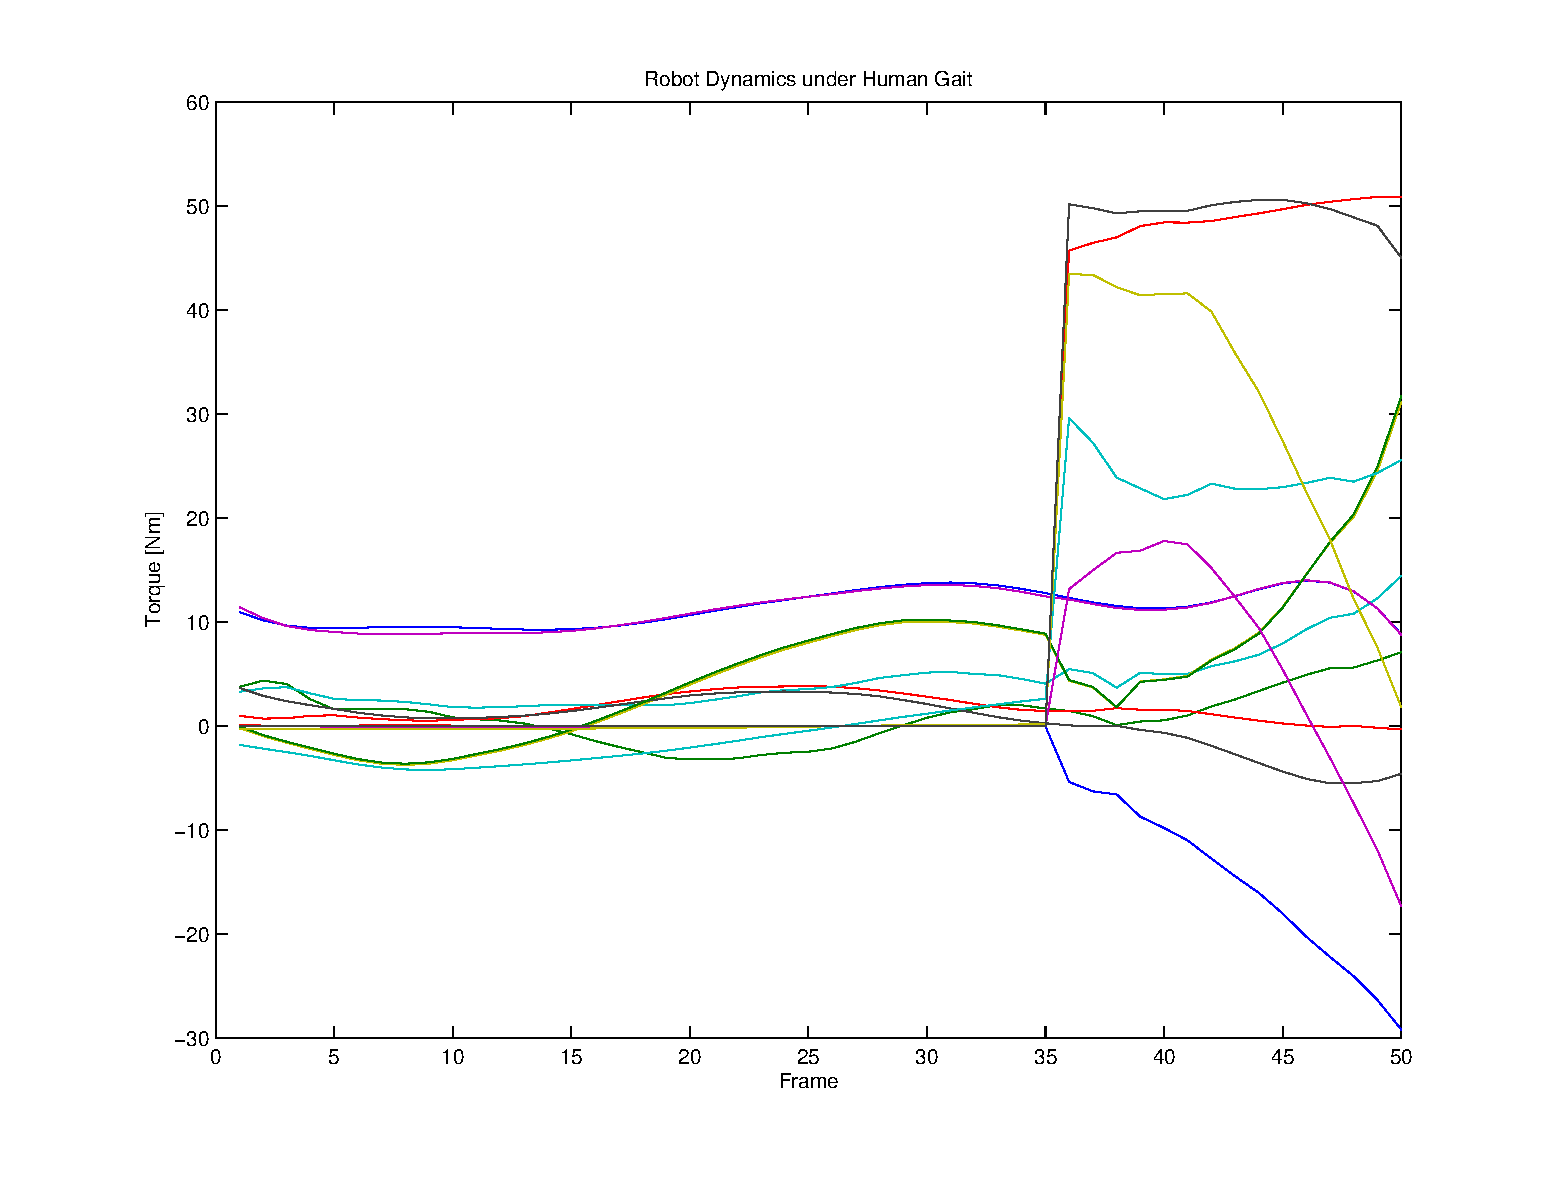
\includegraphics[scale=0.6]{fig/design/gaitplot.eps}
	\end{center}
  \caption{Joint torque profile during the estimated gait cycle obtained from a published data set.}
\end{figure}

Since one of the secondary objectives is to keep the overall mass of the biped as low as possible, it is desirable to select smaller motors where the peak torque loading on the joints are outside of the allowable range of continuous operation. This is a reasonable estimate since the peaks are impulsive forces which only last for a short period of time. The practical approach for deriving specifications from the dynamic simulations is to analyze the continuous torque loading while the system undergoes the gait cycle while keeping the peak loading requirements as a secondary objective. 

\begin{table}[!h]
  \centering
  \caption{Individual joint torque demands for each DOF in one leg using gait estimation.}
    \begin{tabular}{lcc}
    \addlinespace
    \toprule
    \textbf{Joint} & \textbf{Normal} & \textbf{Peak}\\
    \midrule
    Hip Yaw		&	3.698 Nm	&	3.698 Nm\\
    Hip Roll	&	13.606 Nm	&	14.054 Nm\\
    Hip Pitch	&	10.081 Nm	&	38.295 Nm\\
    Knee Pitch  &	5.229 Nm	&	16.539 Nm\\
    Ankle Yaw	&	3.858 Nm	&	3.858 Nm\\
    Ankle Pitch	&	4.395 Nm	&	7.923 Nm\\
    Ankle Roll	&	2.824 Nm	&	5.021 Nm\\
    \bottomrule
    \end{tabular}%
  \label{jointtable}%
\end{table}%

While the torque demands vary for each joint (see Table \ref{jointtable}), the results from the analysis are concatenated to obtain a single set of design specifications. This limit the different models of motors selected from the manufacturer and it also simplifies the electromechanical design process. The combined initial design specifications for the drivetrain components are summarized in Table \ref{tab:spectable}. For the initial design consideration, the normal torque specification is obtained by taking an average of joint torque values during the swing phase. Since the ground reaction forces experienced during the stance phase produce large torques in a short period of time, the peak torque specification is obtained by selecting the highest torque value from all frames. 

\begin{table}[!h]
  \centering
  \caption{Initial design specifications for drivetrain components.}
    \begin{tabular}{lcc}
    \addlinespace
    \toprule
    \textbf{Condition} & \textbf{Torque} & \textbf{Velocity}\\
    \midrule
    Normal & 14 Nm & 2.48 rad/s\\
    Peak  & 50 Nm & 6.82 rad/s \\
    \bottomrule
    \end{tabular}%
  \label{tab:spectable}%
\end{table}%

The contact model parameters (spring and damping coefficients) were observed to have a noticeable effect on the peak design specifications. Since the contact model only provides a crude approximation of the ground reaction forces that the real robot will experience, the final selected value was chosen to provide a peak torque which averages between the largest and smallest values. The final spring and damping coefficients used in deriving the design specifications were $K = 10000$ and $B = 100$, respectively.
% section chassis (end)


%======================================================================
%   D R I V E T R A I N  S E L E C T I O N
%======================================================================


\section{Drivetrain Selection} % (fold)
\label{sec:drivetrain}
The drivetrain selection process includes selecting the appropriate components which transmit the required torque (as per the initial design specifications) to each joint. The electric machines used to generate mechanical power for the purposes of this project are coreless DC motors. The motors used for the 14 DOF bipedal robot were supplied by the Micromo Solutions (part of the Faulhaber Group) \cite{sw:micromo}. The online product catalog was used as a reference tool for the drivetrain selection process. The majority of the weight contribution of the complete system is attributed to the motors. Therefore, the design objective was to select a combination of motor and appropriately sized gearhead to meet the design specifications while keeping the overall mass of the system as low as possible. The remainder of this section presents the selection of appropriate motor and gearhead combination to meet the design objectives. 

\subsection{Mechanical Power Requirements} % (fold)
\label{sub:mechanical_power_requirements}
Similar to most large scale manufacturers of electric machines, Micromo Solutions provide a large catalog of DC motors which are aimed towards a wide variety of applications. To narrow down the selection process into a subset of the motors which meet the initial design specifications, preliminary mechanical power calculations are performed. The mechanical power output required by each generator is specified by the required torque ($\tau$) and speed ($\omega$) of the motor: 

\begin{equation}
	P = \tau \times \omega
\end{equation}

The initial specifications for the drivetrain components listed in Table \ref{tab:spectable} list two values for the torque. As mentioned previously, designing the system to meet the peak torque requirements would yield significantly larger motors and increase the overall mass. Instead, it is desirable to design the system to meet the average (continuous) torque requirements and ensure that the system is capable of withstanding the large impulsive forces experienced at the impact points of the gait cycle. Therefore, the initial mechanical power requirement calculation is based on the normal or average torque loading on the joints (14Nm). While no speed requirements were specified in the initial design specifications, the tabulated kinematic and dynamic data collected from the dynamic simulation was used to compute the average speed experienced by the joints and the largest value was selected for the purposes of calculation. This provides an additional buffer in the mechanical power considerations since not all joints are likely to experience the highest speed. The average speed calculated from the dynamic simulation was found to be 65RPM. Substituting these values along with the conversion factor for units: 

\begin{equation}
	P = \tau \times \omega = 14Nm \times 65RPM \times 0.1047 = 95.28W
\end{equation}

Using this value of mechanical power as a starting guide, the motor catalog is consulted to eliminate the majority of the solutions provided. Note that due to the assumptions placed in calculating this value, 95.28W represents an upper bound on the amount of power the design should be capable of providing. Therefore the potential solution candidates should be rated for the nominal power around the region of this value. The analysis tools presented in the following sections were used to evaluate motor and gearhead combinations from the remaining pool of candidates. Note that only the plots for the final selection is presented as a reference.
% subsection mechanical_power_requirements (end)

\subsection{Torque-Speed Analysis} % (fold)
\label{sub:torque_speed_analysis}
The primary tool used to analyze and compare alternative solutions is the torque-speed graph. Given the structure of the motor specifications provided by Micromo Solutions, a spreadsheet was constructed to automatically generate the torque-speed characteristics from the motor constants. These constants were prepopulated from the manufacturer specification sheets and the torque-speed graphs were automatically. 

\begin{equation}
	\omega = \omega_{no-load} - k\tau
\end{equation}

The relationship between the torque of the motor and the speed of the revolving shaft is approximately linear so it is typically specified by a slope constant for the curve. While the constant $k$ is usually provided as a positive value, the slope of the torque-speed curve is negative (i.e. as the torque increases the speed decreases). 

\begin{figure}[!ht]
	\begin{center}
    \includegraphics[trim = 20mm 30mm 20mm 30mm,clip,width=15cm]{fig/design/motor1.pdf}
	\end{center}
  \caption{Micromo 3257CR Coreless DC Motor: Speed and Current vs Torque}
\end{figure}

% subsection torque_speed_analysis (end)

\subsection{Power and Efficiency Analysis} % (fold)
\label{sub:power_and_efficiency_analysis}
Another key factor in comparing drivetrain components is the relationship between the power produced and the overall efficiency of the motor as a function of its torque. The efficiency curve compares the ratio of electrical power input to mechanical power output. While it is typically desirable to operate the motor at its peak efficiency, the torque demands flactuate throughout the gait cycle making it difficult to base the motor selection process on this premise alone. However, it is desirable to ensure that the motor is reasonably efficient around the intended region of operation. 

\begin{figure}[!ht]
	\begin{center}
    \includegraphics[trim = 20mm 30mm 20mm 30mm,clip,width=15cm]{fig/design/motor2.pdf}
	\end{center}
  \caption{Micromo 3257CR Coreless DC Motor: Power and Efficiency vs Torque}
\end{figure}

% subsection power_and_efficiency_analysis (end)

\subsection{Thermal Analysis} % (fold)
\label{sub:thermal_analysis}
As mentioned previously, out of the initial design specifications the motor selection process is based on the continuous or average torque loading on the joints. However, during each gait cycle the torque demands peak due to external, impulsive force interaction with the environment (i.e. heel-strike). While these peaks may be outside of the motors continuous operating range for a very short period of time, the heat generated inside the motor core can build up and cause significant damage. Another consideration is the effect of thermal build up of the motor under continuous use at the specification of 14Nm. Therefore it is necessary to generate thermal plots alongside the torque-speed analysis to verify that the selected motors can withstand the temperature rise due to its operation. Given an assumed value for the ambient temperature, the total temperature of the motor can be calculated as: 

\begin{equation}
	T_{total} = T_{ambient} + T_{inc}
\end{equation}

Where the temperature increase inside the motor core is provided by the following relationship: 

\begin{equation}
	T_{inc} = I^{2}R \times (R_{th1} + R_{th2})
\end{equation}

Note that $I$ and $R$ is the current through and the resistance of the motor windings, respectively. Constants $R_{th1}$ and $R_{th2}$ are specified by the motor manufacturer. 


\begin{figure}[!ht]
	\begin{center}
    \includegraphics[trim = 20mm 30mm 20mm 30mm,clip,width=15cm]{fig/design/motor3.pdf}
	\end{center}
  \caption{Micromo 3257CR Coreless DC Motor: Speed and Temperature vs Torque}
\end{figure}
% subsection thermal_analysis (end)

\subsection{Final Configurations} % (fold)
\label{sub:final_configurations}
Aside from the torque-speed, power, efficiency and thermal analyses, there are several other factors which come factor in to the design consideration while selecting drivetrain components. These considerations pertain to the secondary objective to minimize the overall weight of the system while simultaneously shifting the COM higher. Between the motor and the gearhead, the majority of the weight comes from the actual coreless DC motor so it is desirable to select a smaller (lighter) motor and meet the specified torque requirements by increasing the gear reduction ratio the gearhead. Another consideration is the physical size of the motor itself, as the diameter and length of each motor vary significantly between different offerings. Since gearheads are coupled directly onto the motor shaft, the complete drivetrain assembly is usually long. 

\begin{figure}[!h]
	\begin{center}
    \includegraphics[trim = 20mm 30mm 20mm 30mm,clip,width=15cm]{fig/design/gearhead1.pdf}
	\end{center}
  \caption{Micromo 38A Precision Gearhead: Speed and Current vs Torque}
  \label{fig:micromo38a}
\end{figure}

Given the considerations and the points of analysis stated in the previous sections, a coreless DC motor from the Micromo Solutions catalog was selected. This motor achieved all of the primary design considerations (average torque requirements, operating within a stable thermal region). Coupled with the motor is a precision gearhead which is capable of producing torques slightly above the initial design specification requirements. The torque-speed characteristics at the gearhead shaft (as shown in Figure~\ref{fig:micromo38a}) is used to verify that the mechanical power output meets the design specification for normal operation. 

While it is desirable to limit the number of different motor and gearhead combinations, it was determined that this combination of drivetrain components was vastly overpowered for the very last joint on the leg (ankle roll). A second combination of motor and gearhead was selected specifically for this joint to reduce the overall mass and raise the COM while meeting the lower joint requirements. This approach improves the controllability of the final system while limiting the total number of different design configurations. The final higher and lower power configurations are defined in Tables \ref{tab:higherconfig} and \ref{tab:lowerconfig}, respectively. 

\begin{table}[!h]
  \centering
  \caption{Higher configuration of motor and gearhead combination from Micromo.}
    \begin{tabular}{lcccc}
    \addlinespace
    \toprule
    \textbf{Model} & \textbf{Mass} & \textbf{Length} & \textbf{Stall Torque} & \textbf{Max Power}\\
    \midrule
    3257CR 12V Motor	&	242g	&	57mm	&	0.547Nm		&	84.50W	\\
    38A 240:1 Gearhead	&	410g	&	80mm	&	20.0Nm		&	-	\\
    \bottomrule
    \end{tabular}%
  \label{tab:higherconfig}%
\end{table}%

\begin{table}[!h]
  \centering
  \caption{Lower configuration of motor and gearhead combination from Micromo.}
    \begin{tabular}{lcccc}
    \addlinespace
    \toprule
    \textbf{Model} & \textbf{Mass} & \textbf{Length} & \textbf{Stall Torque} & \textbf{Max Power}\\
    \midrule
    3242CR 12V Motor	&	172g	&	42mm	&	0.193Nm		&	27.30W	\\
    32A 68:1 Gearhead	&	240g	&	57mm	&	6.0Nm		&	-	\\
    \bottomrule
    \end{tabular}%
  \label{tab:lowerconfig}%
\end{table}%
% subsection final_configurations (end)
% section drivetrain (end)

\section{Mechanical Design} % (fold)
\label{sec:chassis}

The mechanical design of the 14 DOF bipedal robot starts from the initial motor selection presented in the previous section. The 3D CAD models for each motor and gearhead combination is obtained directly from the manufacturer. The design goals for the mechanical chassis are to produce a solid light weight structure which is capable of withstanding external forces from the environment during gait and the applied torques from each joint. The secondary design objective of minimizing the overall weight while shifting the COM higher must also be addressed intrinsically through the mechanical design. 

\subsection{Anthropometric Dimensioning} % (fold)
\label{sub:anthropometric_dimensioning}
The ultimate end goal for the 14 DOF bipedal robot is to achieve walking with human-like gait. To this end, anthropometric dimensioning is used as a starting point for the mechanical chassis design. Starting from a soft height requirement of the full lower body, the relative lengths are obtained for the main linkages (i.e. thigh, shank) from the anthropometric resource shown in Figure~\ref{fig:anthropo}. 

\begin{figure}[!h]
	\begin{center}
    \includegraphics[width=100mm]{fig/design/anthropo.png}
	\end{center}
  \caption{Resource for anthropometric dimensioning of lower body segments \cite{wintergait}.}
\label{fig:anthropo}
\end{figure}
	
Given the ratios between major body segment lengths, a rough estimate for each of the chassis segment lengths is derived and summarized in Table \ref{tab:anthropo}. Note that these dimensions were only used as a starting point. The overall length of the drivetrain components (i.e. motor and gearhead combination) is an additional constraint which can limit how close the final chassis design is to the estimated segment lengths.  

\begin{table}[!h]
  \centering
  \caption{Estimated segment lengths based on anthropometric dimensioning}
  \label{tab:anthropo}%
    \begin{tabular}{lcc}
    \addlinespace
    \toprule
    \textbf{Segment} & \textbf{Height [mm]} & \textbf{Height [In]} \\
    \midrule
    Hip   & 11.32 & 0.45 \\
    Thigh & 277.34 & 10.92 \\
    Shank & 278.47 & 10.96 \\
    Foot  & 44.15 & 1.74 \\
    \bottomrule
    \end{tabular}%
\end{table}

% subsection anthropometric_dimensioning (end)

\subsection{Chassis Structural Design} % (fold)
\label{sub:structural_design}
Aluminum was selected as the light weight rigid material to compose the mechanical chassis for several reasons. The key factors include the widespread availability of various forms of aluminum stock (i.e. channels, beams, etc) and its (relatively) light weight compared to other metal alloys. More specifically, Aluminum 5052 was selected due to its high fatigue strength. While no quantitative stress calculations were performed, this particular attribute is appealing due to the high impact forces the structure will have to absorb with each step. Aluminum 5052 is also easy to work with for manual machining or computer numerical control (CNC) machine tools. 

The chassis is designed as a light weight but rigid frame to house the drivetrain components (actuators, gears, etc). The amount of stock material used in the frame itself also impacts the overall weight and structural rigidity. For example, a link segment designed from a C-Channel beam is structurally sound (since it is a single solid piece of metal). However, it may significantly heavier than a link segment composed of multiple pieces. The trade off between minimizing the overall weight and structural rigidity can sometimes be mitigated by using mechanical design techniques. For example, using a cross brace between adjacent parallel pieces of a frame can significantly improve its structural rigidity while keeping the mass low.  

The lightness of aluminum also helps address the secondary design objective of reducing the overall weight. However, the primary weight contribution to the overall system comes from the drivetrain components. This limits the flexibility for weight manipulation from a purely chassis design standpoint. However, mechanical design techniques can be used manipulate the COM location by strategically positioning the mounting points for motors and gearheads. 
% subsubsection structural_design (end)

\subsection{Mechanical Power Transmission} % (fold)
\label{sub:mechanical_power_transmission}
The biped consists entirely of rotating mechanical joints between link segments. Machine components such as shafts and bearings are used to transmit the rotational mechanical poewr between links. However, this type of mechanical coupling is also used to address the secondary objective of shifting the COM position higher. By using components such as miter gears, the mechanical power transmission is be shifted with a perpendicular offset (90$^\circ$). This technique is used to strategically decouple the mounting position of a drivetrain assembly (i.e. motor with fixed gearhead) from the actual axis of rotation. Consequently, this decoupling is used to relocate motors in a way such that the weight distribution is manipulated in favour of having a higher COM position (illustrated in Figure \ref{fig:miter}).
	
\begin{figure}[!h]
	\begin{center}
    \includegraphics[scale=0.5]{fig/design/perpendicular.pdf}
	\end{center}
  \caption{Perpendicular mechanical coupling to shift weight distribution.}
\label{fig:miter}
\end{figure}

Mechanical coupling and power transmission is also used to design  intersecting axes of rotation. By using spur gears with a 1:1 reduction ratio, the output shaft of a drivetrain assembly can be positioned in a parallel offset (illustrated in Figure \ref{fig:spur}).

\begin{figure}[!h]	
	\begin{center}
    \includegraphics[scale=0.5]{fig/design/parallel.pdf}
	\end{center}
  \caption{Parallel mechanical coupling to allow intersection axis of rotation.}
\label{fig:spur}
\end{figure}

Shafts are frequently used to enable rotation between two link segments in the mechanical design. Ball bearings are common machine components which support the rotational movement of these shafts within a solid frame chassis. Traditional shielded ball bearings were selected for joints to support radial loads while permitting the rotation of a shaft on the inner ring (as illustrated in Figure \ref{fig:ballb}). The double shielded construction provides protection against debris from entering the bearing assembly without producing significant internal friction forces that are present in the case of sealed bearings. 

\begin{figure}[!h]
	\begin{center}
    \includegraphics[scale=0.5]{fig/design/ballbearings.pdf}
	\end{center}
  \caption{Enabling rotational motion of shafts using double shielded ball bearings.}
\label{fig:ballb}
\end{figure}

For yaw joints which actuate along the vertical axis, the impact forces experienced during the gait cycle exert an axial load which is typically not supported by traditional ball bearings (would cause the inner ring to ``pop out''). Furthermore, these joints experience axial loads in one direction while the robot is standing on the ground but the load reverses direction if the robot is picked up by the torso. Therefore, bidirectional support for axial loads is required for the hip and ankle yaw joints. For these sections of the lower body, a combination of thrust and ball baerings are used to support radial and axial loads (as shown in Figure~\ref{fig:yawbearing}. 

\begin{figure}[!ht]
	\begin{center}
    \includegraphics[trim = 5mm 34mm 5mm 25mm,clip,width=15cm]{fig/design/yawbearing.pdf}
	\end{center}
  \caption{A combination of thrust and ball bearings used for yaw joints to support radial and axial loading.}
\label{fig:yawbearing}
\end{figure}

% subsubsection mechanical_power_transmission (end)

% section mechanical_design (end)

\section{Summary} % (fold)
\label{sec:design_summary}
The electromechanical design of the 14 DOF bipedal robot had two primary design objectives. The first was to produce enough mechanical power for the biped to achieve walking. The secondary design objective to keep the overall weight low and raise the COM improves the controllability of the final design. The initial design process started from the basics of dynamic modeling of multibody systems. The forward and inverse dynamic models computed with the RNE algorithm provided a mathematical framework for estimating the torque requirements at each joint. 

Since the end goal is to develop a biped capable of human-like walking, a published dataset of motion captured human gait was used for the initial dynamic simulation. Using MATLAB toolboxes, the kinematic constraints on each joint ($\vec{q}$, $\vec{\dot{q}}$, $\vec{\ddot{q}}$) were imposed on the dynamic model of the biped. A spring-damper contact model was used to generate an approximate ground reaction force experienced by the biped while walking. Finally, the initial joint torque and velocity demands under the estimated gait cycle were obtained through the dynamic simulations. 

These initial design specifications formed the basis for drivetrain selection. The primary design goal of producing enough mechanical power for bipedal locomotion was addressed by appropriately sizing electric machines to the specifications. A combination of DC motors and precision gearheads were evaluated by analyzing the torque-speed, power, efficiency and thermal characteristics. The selection process revealed that a set of high and low power configuration of drivetrain components would meet the specifications while minimizing the overall weight of the system. 

After the drivetrain configurations were established, the secondary design goal of minimizing the overall weight and raising the COM were addressed intrinsically through the mechanical design in CAD. A rough guideline for dimensioning the lower body segments (i.e. thigh, shank) was obtained through anthropometric dimensioning and the desired height of the lower body. Aluminum 5052 was selected as the material to construct the chassis frame due to its light weight, fatigue strength and machineability. The power transmission system (composed of shafts, bearings and gears) connecting the actuators to the linkages were strategically designed to raise the COM and support the loading during gait. 

This concluded the initial prototype design of the 14 DOF bipedal robot in CAD. Further improvements to the mechanical design (i.e. adjusting link lengths or motor positioning) and analysis of the electromechanical system under control action required dynamic simulations. The following chapter presents a rapid prototyping toolchain for accomplishing these objectives with minimal user input. 
% section discussion (end)

% chapter design (end)
    \chapter{Toolchain Development} % (fold)
\label{cha:toolchain}
The electromechanical design and development of multibody robotic systems is an iterative process, starting from a mechanical model in Computer Aided Design (CAD) software, transferring its parameters to a dynamic simulator for analysis and revising the design to improve the performance of the system. This process is repeated until the mechanical design achieves some desired goal. The iterative nature of the design and analysis process can often become time consuming and cumbersome. However, for high degree of freedom (DoF) multibody systems, the iterative approach is necessary as small changes in the mechanical design can have a significant impact on the overall dynamics of the system and the resulting system behaviour as well as implications for control design. Another popular approach is the use of optimization tools \cite{Paul2001,Wollherr2002} to determine the optimum design configuration. However, the resulting configuration may not be realizable with the available hardware components and must still be verified in simulation before hardware implementation.

There exists a wide variety of dynamic simulation environments with a range of capabilities \cite{Koenig04designand,michel2004webotstm, Kanehiro:2004dq, PonticelliCWR2006, Reichenbach2009, MedranoCerda2010}. These environments provide a feature complete package, which combine an underlying dynamics engine with an interface for visualizing the simulations. The underlying computation engines obtain the complete equations of motion for the system described by its kinematic/dynamic parameters using techniques including, but not limited to, Lagrange multipliers \cite{Baraff1996}, Kane's method \cite{Rosenthal1986} and port-based modeling \cite{Paredis2001}. The equations of motion are integrated to obtain the system state at each time step. Most simulators provide support for importing common Virtual Reality Markup Language (VRML) or Standard Tessellation Library (STL) files generated by CAD tools for visualization \cite{Koenig04designand,michel2004webotstm}. However, only a few provide direct compatibility with CAD tools to import kinematic/dynamic parameters for simulation.

Open Architecture Humanoid Robotics Platform (OpenHRP) \cite{Kanehiro:2004dq} is a commonly used dynamic simulation environment for humanoid robots that supports importing VRML files. However, kinematic and dynamic parameters of the robot are specified as plain text, making it cumbersome for rapid iterations.

MapleSim \cite{sw:maplesim}  is a multibody simulation package that provides limited functionality to communicate with CAD applications through its MapleSimConnector toolbox. This toolbox uses the underlying Maple engine with command-line access for retrieving the parameters of each link. However, the CAD application has to be actively running in the background and it is left to the user to generate Maple worksheets for batch importing of the parameters to update the link parameters in MapleSim through its API.

SimMechanics \cite{sw:simmech} provides mechanical import functionality to generate Extensible Markup Language (XML) files containing link parameters directly from CAD along with the corresponding STL files for visualization. However, there are limitations on how joint constraints are defined in CAD to successfully generate an equivalent model in Simulink. Another drawback of this approach is that the visualization generated during simulations significantly impacts the simulation speed.


\section{CAD Export} % (fold)
\label{sec:cad_export}

% section introduction (end)
We developed an add-in for CAD software package SolidWorks to export a multibody system for dynamic simulations in Simulink with realtime visualization. Consider a standard multibody system with $n$ joints and $n + 1$ links. The links are numbered from 0 (base) to $n$ and each $joint_{i}$ connects $link_{i-1}$ to $link_{i}$.

The mechanical design of each link is represented by its own CAD assembly (or part) file. The coordinate system at the origin of this CAD file is treated as the local coordinate system $xyz_{i}$ rigidly attached to the link $i$.

The top most CAD assembly (referred to as the \emph{master assembly}) contains all $n + 1$ links as subassembly files connected and constrained by the mechanical relationship which defines the behaviour of each joint $n$. For example, a revolute joint connecting two link subassemblies is defined by the appropriate constraints (i.e. concentric relationship).

\begin{figure}[!b]
	\centering
    \includegraphics[scale=0.7]{fig/ch3/exporter.png}
  	\caption{Our exporter add-in for SolidWorks (named Quanser Exporter in the SolidWorks tab) to capture relevant physical and visualization data.}
	\label{fig:swexporter}
\end{figure}

Our add-in for SolidWorks uses this master assembly file as a starting point to export the multibody system for dynamic simulations. Once installed, a new tab is added directly in SolidWorks (as shown in Figure \ref{fig:swexporter}) presenting the user with several export options. The initial export process prompts the user with a flat list of all subassemblies in the current file via a \emph{Model Organizer} interface (shown in Figure~\ref{fig:modelorg}). Each subassembly is treated as a node that can be ordered (through a drag-and-drop interface) to form the desired kinematic tree/chain hierarchy. 


\begin{figure}[!t]
	\centering
    \includegraphics[scale=0.60]{fig/ch3/modelorg.png}
  	\caption{The \emph{Model Organizer} window used to define the kinematic structure of the system during initial export.}
	\label{fig:modelorg}
\end{figure}

\subsection{Physics Export} % (fold)
\label{sub:physics_export}
Each link subassembly is parsed in the order defined in the \emph{Model Organizer} window to extract key kinematic/dynamic parameters. All numerical values (i.e. distance between links) are extracted directly using CAD tools.

Assuming that the system is in the home configuration at the time of export, the relative frame transformations $T^{i-1}_{i}$  between subsequent frames are extracted in accordance with the kinematic hierarchy defined in the \emph{Model Organizer}. The absolute frame transformations $T^{0}_{i}$ are also computed with respect to the base link (if the base link is fixed in the master assembly file). For floating base systems (i.e. base link has 6 DOF), the absolute frame transformations $T^{W}_{i}$ are taken with respect to the coordinate system of the master assembly file (world frame). The mass and dynamic properties are extracted with internal CAD tools in the local coordinate system of the link subassembly file. The mass, distance to the center of mass (COM) and inertia tensor of the link (at the COM position) are extracted.

Our add-in captures these key parameters and generates a structured XML file. A XML node is generated for each link containing the extracted kinematic/dynamic parameters (as shown in Figure \ref{fig:exportfile}). Furthermore, each XML link node is organized in accordance with the kinematic hierarchy of the system. As a result, our add-in captures the entire physical description of the multibody system in a portable, language independent file.

\begin{figure}[!b]
	\centering
    \includegraphics[scale=0.4]{fig/ch3/exportfile.png}
  	\caption{Example of kinematic and dynamic parameter extraction straight from CAD model stored in the exported XML file.}
	\label{fig:exportfile}
\end{figure}

% subsection physics_export (end)

\subsection{Mesh/Scene Export} % (fold)
\label{sub:mesh_scene_export}

In addition to exporting the physical description of the model, our exporter add-in also generates files for visualization. These files can be used in conjunction with dynamic simulations to provide the user with visual feedback of the system under control. Some dynamic simulators (SimMechanics, MapleSim) currently allow users to specify a VRML file for each link of the multibody system. While SolidWorks currently has some support to export VRML files for each link subassembly individually, there are no options to generate the 3D meshes in X3D (successor to VRML).

We have developed a process for automated batch generation of full 3D meshes in the X3D format. Once the export process has been initiated, the meshes are extracted for each link subassembly in the master assembly file directly from the CAD layout. Each mesh is aligned with the local coordinate system of the link such that there is a direct mapping between the visualization and the physical model.

The overall mesh generation process is optimized for complex multibody systems. A typical CAD subassembly representing each link may contain hundreds of smaller CAD part/assembly files. During the mesh generation process our add-in creates a new flattened version of each link subassembly and discards any visual details not visible on the surface. The surfaces of this flattened model are tessellated to generate the mesh file for each link. As a result, the mesh files are light weight and this helps speed up the rendering process. At the time of writing, our toolset does not yet provide the user with the ability to specify the level of detail for tessellation.

The output mesh files are stored in the same directory as the XML file containing the physical description of the system. Furthermore, each link XML node is also updated with a complete path to its corresponding mesh file alongside the kinematic/dynamic parameters.

Our add-in also generates a \emph{scene} file from the CAD master assembly. This is a parallel XML file which contains a complete visual description of the system from CAD. The scene file contains a list of all links alongside their corresponding mesh files. These meshes are then organized in accordance with the kinematic tree/chain hierarchy provided by the user in the \emph{Model Organizer}.

As a result, the scene file recreates the visual layout of the complete multibody system from the CAD master assembly file. This file encapsulates the full multibody system in a format which is compatible with the 3D visualization blocks that are packaged with the QUARC toolbox. In addition to the model itself, additional supplementary mesh files (i.e. ground plane) are imported into the scene for visualizing the environment during simulation.
% subsection mesh_and_scene_export (end)

\subsection{CAD Update} % (fold)
\label{sub:cad_update}

With minimal user input, our add-in captures a complete physical and visual description of the system in its \emph{current state}. However, the main benefits of our approach become apparent after the initial export. Once the user defines the structure of the system (kinematic hierarchy and joint definitions) through the \emph{Model Organizer}, it is stored in memory for later use. Subsequent updates to the CAD model can be exported with a single click if the overall structure of the links and joint definitions do not change.

This allows the user to export a model for simulation from CAD, analyze the behaviour of the system under control, tweak the mechanical design and immediately re-export the revised model for simulation. For example, increasing the length of a link may alter its dynamic properties  while the overall kinematic structure remains the same. The revised CAD model with increased link length can be exported with a single click. The export process simply recalls the structure of the system and regenerates the XML files with updated kinematic/dynamic properties. Our add-in also allows the user to regenerate only the mesh file for the updated link to reflect the changes in CAD. This process makes it fast and easy for rapid iterations during the design phase.
% subsection cad_update (end)

% section cad_export (end)

\section{Model Generation} % (fold)
\label{sec:model_generation}
The XML files exported by our add-in encapsulate the relevant information which describes the CAD model into structured and portable files. One of the key advantages of our approach is that the information in these files can easily be parsed to generate an equivalent model in most dynamic simulators. We have developed a model generation counterpart for the Matlab/Simulink environment which uses SimMechanics for multibody dynamic simulation and Quanser's QUARC toolbox for 3D visualization. This provides a semi-automated toolchain for designing robotics and/or mechatronic systems.

Our model generation approach provides several Matlab functions, scripts and libraries to parse the files exported by our SolidWorks add-in and generate the equivalent mechanical system in Simulink. The generated Simulink model contains (a) SimMechanics blocks with the link kinematic and dynamic parameters from CAD and (b) visualization blocks from QUARC libraries with the link meshes and scene file. The generated physics and visualization counterpart is prepopulated with CAD data and connected according to the kinematic hierarchy of the system defined in the \emph{Model Organizer}.

The model generation process is initiated by calling a function in the Matlab terminal inside the CAD export folder. By default, our approach generates a physical subsystem (i.e. the “plant”) for forward dynamics simulation, whose output drives a generated visualization subsystem. The user can also generate an inverse dynamics model through the command line.

\subsection{Physical Model} % (fold)
\label{sub:physical_model}

\begin{figure}[!b]
	\centering
    \includegraphics[scale=0.50]{fig/ch3/simmech.pdf}
  	\caption{Our standard link subsystems for physical model generation with prepopulated kinematic and dynamic parameters from CAD.}
	\label{fig:quarcmech}
\end{figure}

Our physical model generation process parses the XML output files in the export folder to create a CAD-equivalent system in Simulink. In order to streamline the process, we have developed a library (shown in Figure \ref{fig:quarcmech}) of masked link subsystems representing common link configurations. Each of these subsystems contains a combination of SimMechanics joint, body, actuator and sensor blocks to represent a combination of $joint_{i}$ and $link_{i}$ (shown in Figure \ref{fig:undermask}).

\begin{figure}[!t]
	\centering
    \includegraphics[scale=0.38]{fig/ch3/undermask.pdf}
  	\caption{SimMechanics blocks used to compose each CAD-equivalent link subassembly in Simulink}
	\label{fig:undermask}
\end{figure}

The input to each link subsystem (\textbf{CS1}) is a connection from $link_{i-1}$ and the driving signal for the joint. The output of the link subsystem is its local coordinate system (\textbf{CS2}) and the joint sensor signals. The joint actuator/sensor signals are set depending on the type of dynamic simulation. By default the model generation process configures the physical model in forward dynamics mode so the joint actuator port is connected to the force/torque command input for $joint_{i}$ and joint angle/displacement is measured at the output. Alternatively, for the inverse dynamics simulation, the joint acceleration is set as the input, while the joint force/torque is the output.

The output coordinate system of the $joint_{i}$ block is connected to a SimMechanics body block representing $link_{i}$. The masked parameters are preconfigured to set the local dynamic properties (i.e. COM position, inertia tensor) and relative frame transformation appropriately.

Each link subassembly from CAD is recreated with a link subsystem from our library depending on the link type. The masked parameters are populated with the kinematic and dynamic parameters from the corresponding XML link node. The overall hierarchy of links is parsed and each link subsystem is connected accordingly. Our model generation process also automatically handles the signal routing from the input/output ports of the physical model. In the default forward dynamics configuration, the $n \times 1$ torque/force vector is connected to all joint actuator blocks and the output signals from the sensors are also routed accordingly. For the inverse dynamics case, the vector of joint positions, velocities and accelerations are connected to the joint actuator blocks and the sensors are preconfigured to output the resulting torque/force vector.

In addition to the link subsystem, a ground block representing the coordinate frame of the CAD master assembly is connected to the base $link_{0}$. The entire process of creating an equivalent model for dynamic simulation is automated. The user simply calls the appropriate function and the generated physical model subsystem is placed in a new (or existing) Simulink diagram.
% subsection physical_model (end)

\subsection{Visualization Model} % (fold)
\label{sub:visualization_model}
Our visualization model generation process generates a single subsystem containing blocks to initialize and drive the scene file generated from CAD. The mesh for each link in the kinematic chain is driven by the output of the generated physical model (forward dynamics subsystem) so that there is a 1:1 mapping between the plant and what is being rendered by the visualization. When a simulation is running, an external 3D viewer application (part of the QUARC toolbox) is used to render the scene in realtime using OpenGL (CAD-equivalent visualization scene file shown in Figure \ref{fig:masterscene}).

\begin{figure}[!t]
	\centering
    \includegraphics[scale=0.40]{fig/ch3/masterscene.pdf}
  	\caption{CAD master assembly shown on the left is used to automatically generate the meshes and scene file to recreate the visualization shown on the right.}
	\label{fig:masterscene}
\end{figure}

Our approach allows the user to receive immediate visual feedback of the CAD model under the influence of control. This also allows the user to make changes to the mechanical design from visual observations (i.e. quick changes to improve joint limits).
% subsection visualization_model (end)

\subsection{Model Update} % (fold)
\label{sub:model_update}
Our export add-in makes it possible to make changes to the mechanical design in CAD and generate the new kinematic and dynamic parameters immediately. After the initial model generation from CAD data, these new changes can be reflected back into the dynamic simulation by simply calling the update function. The update functionality also allows the user to specify the path to the previously generated physical model. The masked parameters on each link subsystem inside this model are simply updated with the new changes while the signal routing and everything else is left intact. The updated mesh files are loaded by the QUARC 3D viewer during the next simulation run.

This streamlines the iterative design process by allowing a user to export a system from our add-in and generate the CAD-equivalent physical/visual model in Simulink. The behaviour of the system can then be analyzed in dynamic simulations to revise the CAD design. Once the new changes are applied, the revised parameters are easily exported back into dynamic simulations for further analysis.
% subsection model_update (end)

% section model_generation (end)

% chapter toolchain (end)

    \chapter{Simulation Work} % (fold)
\label{cha:simulations}
In thesis, the 2D FPE theory is extended for 3D bipedal robots by selecting a sagittal plane in 3D space and constraining the swing foot motion within this plane. Once the biped is unstable, we solve FPE equation along the selected plane to determine the swing foot placement to ultimately regain stability. Similar to the approach used in \cite{Wight:2008ii,Wight:2008vt}, we extend this concept to form complete gait cycles with a state machine, high gain PD controllers and no precomputed trajectories.


\section{Whole Body Control} % (fold)
\label{sec:whole_body_control}
Lorem ipsum dolor sit amet, consectetur adipisicing elit, sed do eiusmod
tempor incididunt ut labore et dolore magna aliqua. Ut enim ad minim veniam,
quis nostrud exercitation ullamco laboris nisi ut aliquip ex ea commodo
consequat. Duis aute irure dolor in reprehenderit in voluptate velit esse
cillum dolore eu fugiat nulla pariatur. Excepteur sint occaecat cupidatat non
proident, sunt in culpa qui officia deserunt mollit anim id est laborum.
% section whole_body_control (end)

% chapter simulations (end)
    \chapter{Experimental Results} % (fold)
\label{cha:experiments}

This chapter presents the experimental work completed to validate the actuator dynamics and motion control framework used in simulation. It is important to test walking control strategies on physical hardware directly due to the imperfections in a simulation environment. For example, the contact models used to estimate the ground reaction force is only an approximation. There are also other unmodeled effects which can significantly alter the dynamics of the physical system (i.e. vibrations). The simulations used to demonstrate the proposed 3D FPE walking control strategy in the previous section was designed to account for link side dynamics only. Section~\ref{sec:actuator_model} describes the modifications to account for the actuator dynamics. This modification to the simulations enables a single controller designed in Simulink to target either the simulation environment or the physical hardware using the HIL architecture discussed in Section~\ref{sec:hil_architecture}. The experimental validation for a single actuator and the proposed motion control framework are presented in Sections \ref{sec:1dof_validation} and \ref{sec:motion_control_validation}, respectively. 

\section{Actuator Model} % (fold)
\label{sec:actuator_model}
In the ideal case, the control signal $\vec{u}$ applied to each joint would simply be $\vtau$ shown on the right hand side of (\ref{eq:eom1}). However, 

\begin{figure}[!h]
	\centering
    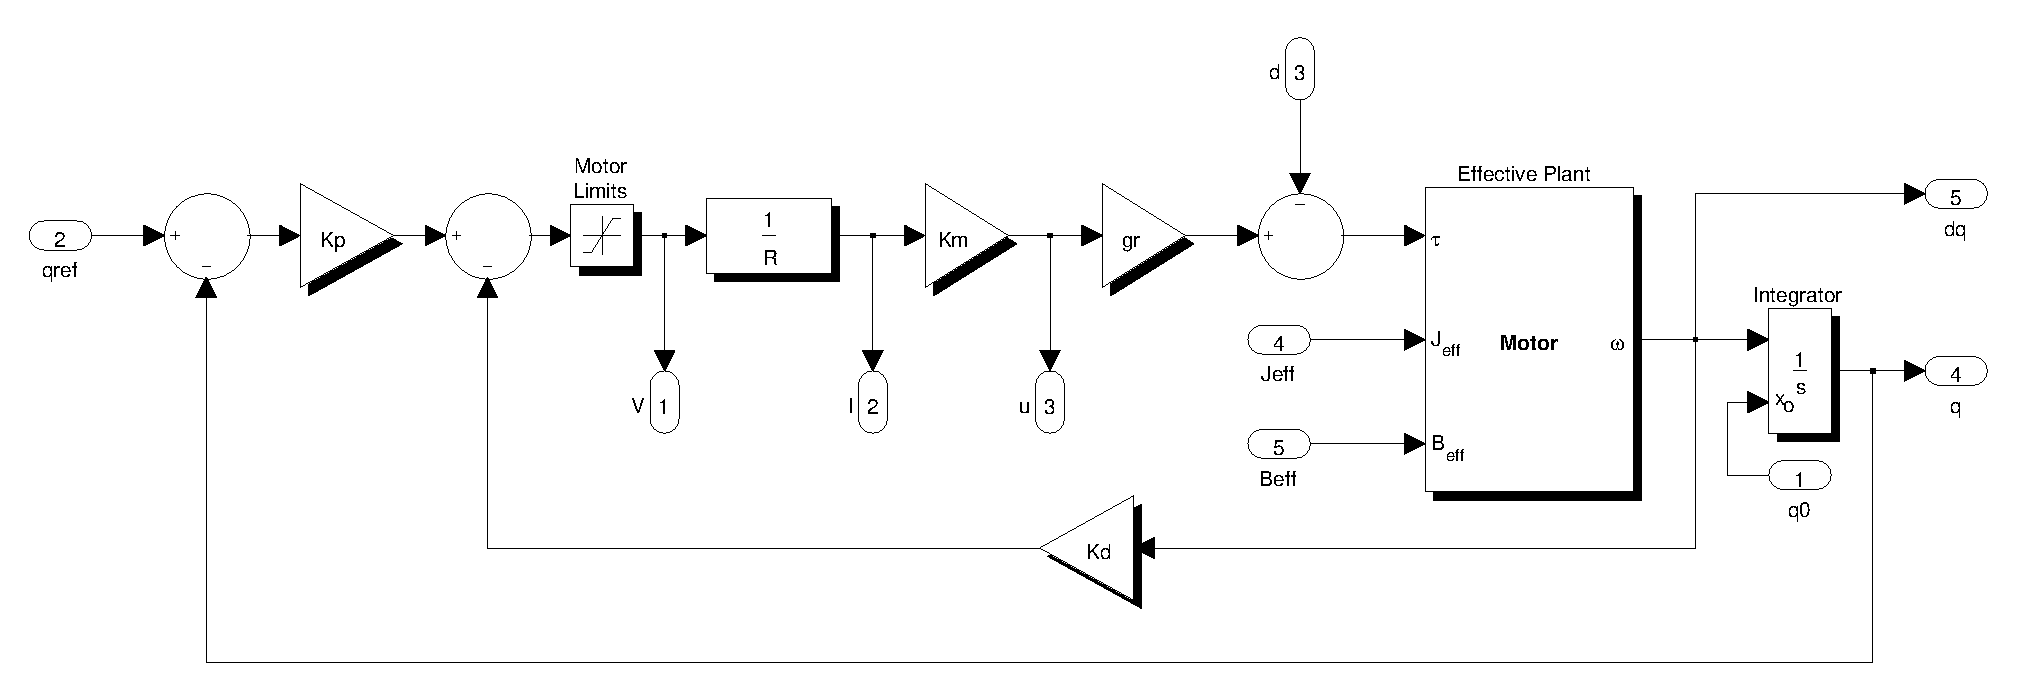
\includegraphics[scale=0.5]{fig/experiments/pdmotorcontroller.eps} 
  	\caption{PD Controller implementation for independent joint control with actuator dynamics.}
	\label{fig:pdmotorcontroller}
\end{figure}

% section actuator_model (end)

\section{HIL Architecture} % (fold)
\label{sec:hil_architecture}
Incomplete. 

\begin{figure}[!h]
	\centering
    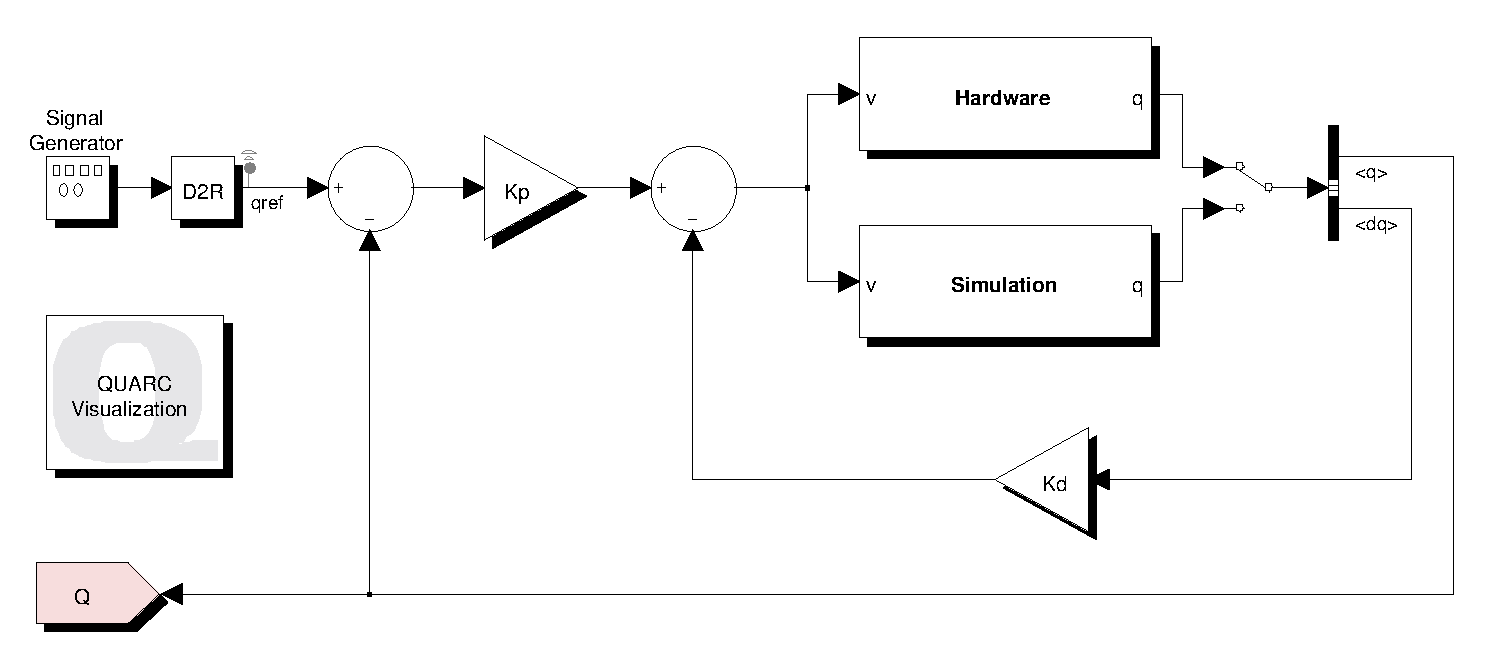
\includegraphics[scale=0.6]{fig/experiments/parallelmodels.eps} 
  	\caption{Parallel models designed to target either simulations or physical hardware with the same controller.}
	\label{fig:parallelmodels}
\end{figure}

\begin{figure}[!h]
	\centering
    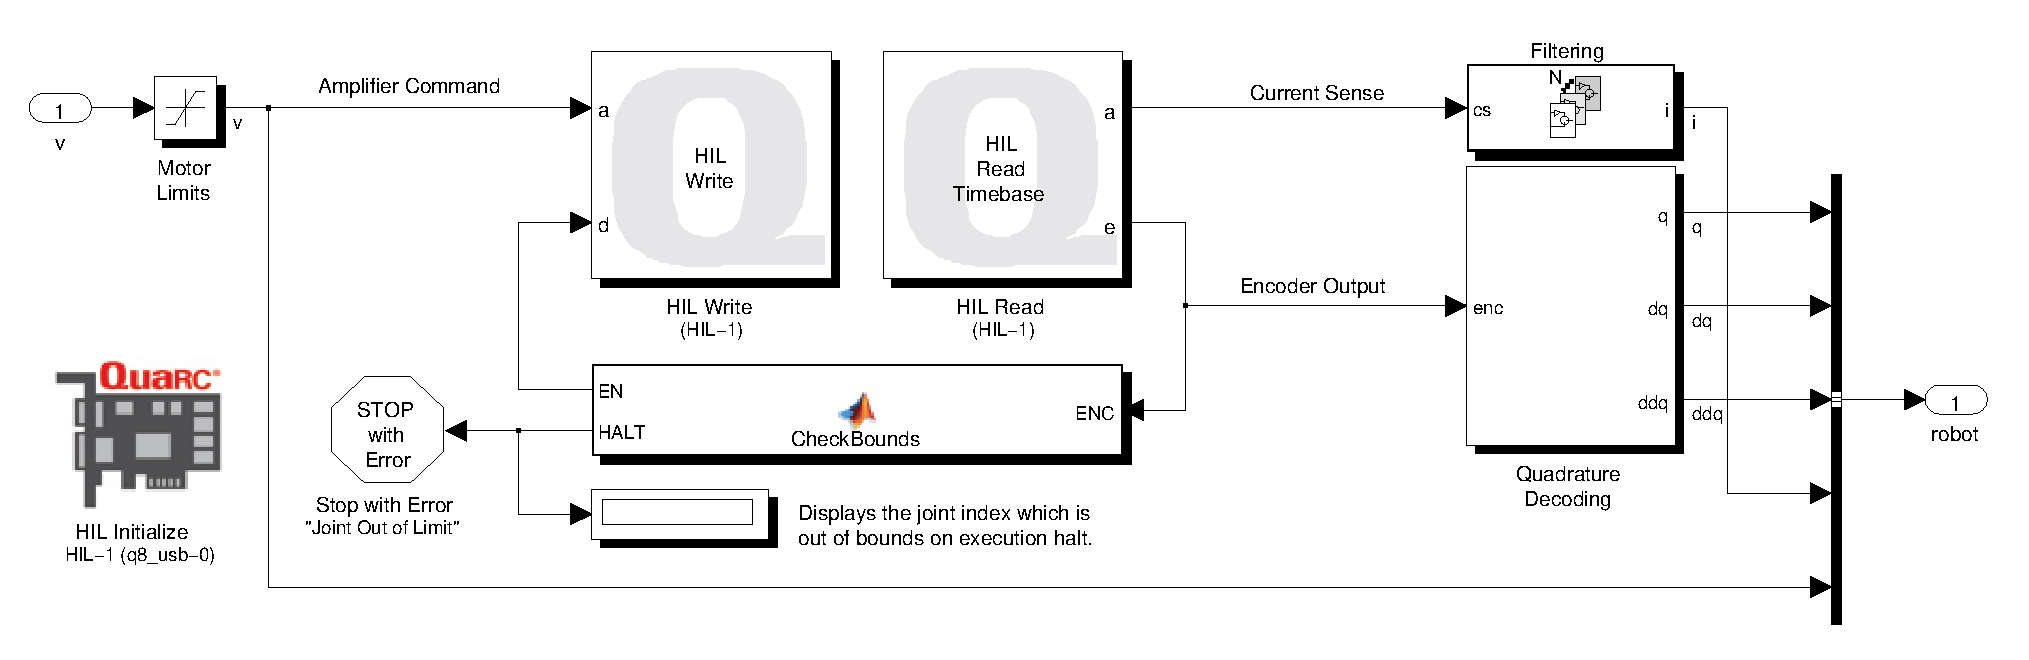
\includegraphics[scale=0.45]{fig/experiments/hilmodel.eps} 
  	\caption{HIL subsystem from Figure~\ref{fig:parallelmodels} used to target physical hardware with voltage control signal.}
	\label{fig:hilmodel}
\end{figure}

\begin{figure}[!h]
	\centering
    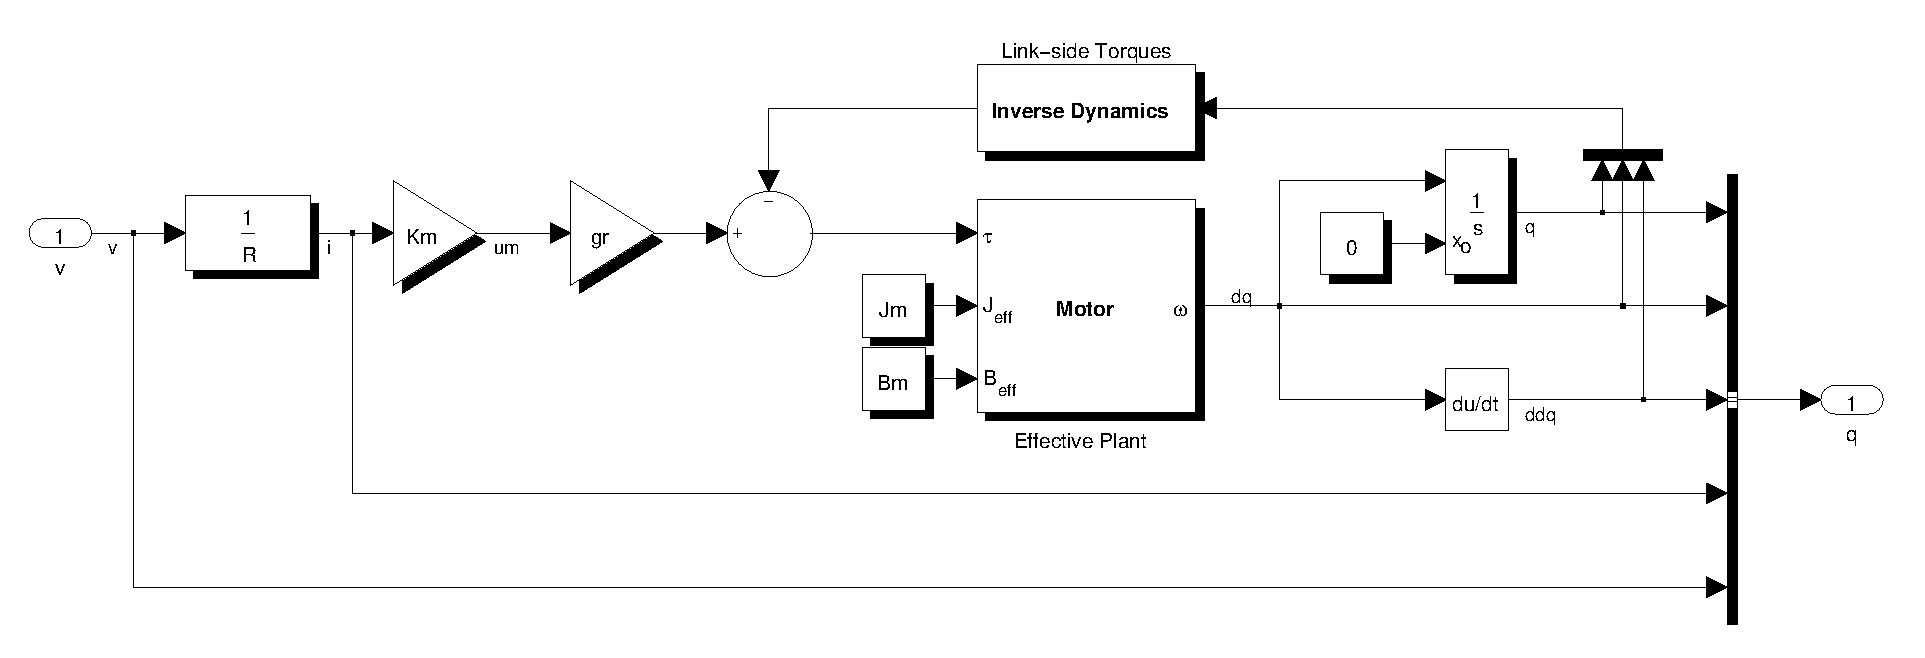
\includegraphics[scale=0.55]{fig/experiments/simmodel.eps} 
  	\caption{Subsystem from Figure~\ref{fig:parallelmodels} used to target the simulated environment with voltage control signal.}
	\label{fig:simmodel}
\end{figure}

% section hil_architecture (end)

\section{Single DOF Validation} % (fold)
\label{sec:1dof_validation}
Incomplete. 
% section 1dof_results (end)

\section{Motion Control Validation} % (fold)
\label{sec:motion_control_validation}
\Incomplete. 
% section motion_control_results (end)

\section{Discussion} % (fold)
\label{sec:experiments_discussion}
Incomplete. 
% section discussion (end)

% chapter experiments (end)
    \chapter{Conclusions} % (fold)
\label{cha:conclusion}
\ifthenelse{\boolean{VoidIncomplete}}{\Incomplete}{

Lorem ipsum dolor sit amet, consectetur adipisicing elit, sed do eiusmod
tempor incididunt ut labore et dolore magna aliqua. Ut enim ad minim veniam,
quis nostrud exercitation ullamco laboris nisi ut aliquip ex ea commodo
consequat. Duis aute irure dolor in reprehenderit in voluptate velit esse
cillum dolore eu fugiat nulla pariatur. Excepteur sint occaecat cupidatat non
proident, sunt in culpa qui officia deserunt mollit anim id est laborum.

\section{Future Work} % (fold)
\label{sec:future_work}
Lorem ipsum dolor sit amet, consectetur adipisicing elit, sed do eiusmod
tempor incididunt ut labore et dolore magna aliqua. Ut enim ad minim veniam,
quis nostrud exercitation ullamco laboris nisi ut aliquip ex ea commodo
consequat. Duis aute irure dolor in reprehenderit in voluptate velit esse
cillum dolore eu fugiat nulla pariatur. Excepteur sint occaecat cupidatat non
proident, sunt in culpa qui officia deserunt mollit anim id est laborum.


% FROM SECTION 5.3.1: 

The use of variable step solvers was explored as an option to reduce simulation runtime while providing a stiffer ground with much higher contact model constants. 


% section future_work (end)
}
% chapter conclusion (end)

    % B A C K   M A T T E R
    %======================================================================
%   B A C K  M A T T E R
%======================================================================


% B I B L I O G R A P H Y
% -----------------------
\bibliographystyle{plain}
\cleardoublepage 
\phantomsection

\renewcommand*{\bibname}{References} % Use "References" instead of "Bibliography"
\addcontentsline{toc}{chapter}{\textbf{References}} % Add the References to the Table of Contents

\bibliography{bib/masc-thesis}
\nocite{*}


% A P P E N D I C E S
% -------------------
% \appendix
% \chapter*{Appendices} % Add a title page before the appendices and a line in the Table of Contents
% \addcontentsline{toc}{chapter}{Appendices}

% \input{tex/appendix-a}

\end{document}

\bye
